%----------------------------------------------------------------------------------------
%	PACKAGES AND OTHER DOCUMENT CONFIGURATIONS
%----------------------------------------------------------------------------------------

\documentclass[11pt, a4paper, oneside]{Thesis} % Paper size, default font size and one-sided paper

\graphicspath{{./figures/}} % Specifies the directory where pictures are stored

\usepackage[square, numbers, comma, sort&compress]{natbib} % Use the natbib reference package - read up on this to edit the reference style; if you want text (e.g. Smith et al., 2012) for the in-text references (instead of numbers), remove 'numbers' 
\hypersetup{urlcolor=black, colorlinks=true} % Colors hyperlinks in blue - change to black if annoying
\title{\ttitle} % Defines the thesis title - don't touch this

\usepackage{tikz}
\usepackage{setspace}

\definecolor{OrangeGSSI}{RGB}{237,113,45}
\definecolor{blue}{RGB}{25,25,112}

%----------------------------------------------------------------------------------------
%	DOCUMENT VARIABLES
%	Fill in the lines below to update the thesis template
%	If you wish to cite each of the variables defined below, look at the
%	section above for the citation command e.g. \examiner{} below is
%	defined as \examname above so you cite it as \examname
%----------------------------------------------------------------------------------------

\thesistitle{Topological and Numerical Stability of Higher-Order Laplacian Operators on Simplicial Complexes} % Your thesis title - this is used in the title and abstract
%-------------------------------------------------  
\supervisor{Prof.~Francesco~\textsc{Tudisco} and Prof.~Nicola~\textsc{Guglielmi}} % You supervisor's name - this is used in the title page
%-------------------------------------------------   
\examiner{Dr. Name  \textsc{Surname}} % Your examiner's name - this is not currently used anywhere in the template, cite it with \examname if you want it
%-------------------------------------------------   
\degree{Doctor of Philosophy} % Your degree name - this is currently used in the title page and abstract
%-------------------------------------------------   
\authors{Anton \textsc{Savostianov}} % Your name - this is used in the title page and abstract
%-------------------------------------------------

%----------------------------------------------------------------------------------------
%	TYPESETTING
%----------------------------------------------------------------------------------------
\usepackage{pifont}
\usepackage{xcolor,colortbl}
\usepackage{flushend}
\usepackage[normalem]{ulem} % for \sout
\usepackage{multicol}
\usepackage{xcolor}
\newcommand{\ugh}[1]{\textcolor{red}{\uwave{#1}}} % please rephrase
\newcommand{\ins}[1]{\textcolor{blue}{\uline{#1}}} % please insert
\newcommand{\del}[1]{\textcolor{red}{\sout{#1}}} % please delete
\newcommand{\chg}[2]{\textcolor{red}{\sout{#1}}{\ra}\textcolor{blue}{\uline{#2}}} % please change

\renewcommand{\ttdefault}{cmr}

\newcommand{\assignedto}[1]{\textcolor{red}{\ding{46}~{\sf Assigned to:}~#1}\\}
\newcommand{\todo}[1]{\textcolor{blue}{\ding{46}{\sf}~#1}}

\newcommand{\sugg}[1]{\textcolor{orange}{#1}}
%----------------------------------------------------------------------------------------
%	End of TYPESETTING
%----------------------------------------------------------------------------------------


\usepackage{tikz-network}
\usepackage{faktor}


%%%% COMMANDS %%%%%%%%%%%%%%%%%%%%%%%%

\newcommand*{\insidefigure}[3][0.5\columnwidth]{
      \begin{center}
            \begin{minipage}{#1}
                  \centering
                  #2
                  \captionof{figure}{#3}
            \end{minipage}
      \end{center}
}

\newcommand*{\mc}[1]{\mathcal{#1}}
\renewcommand*{\b}[1]{\mathbf{#1}}
\newcommand*\eps{\varepsilon}
\newcommand*{\V}[1]{ \mc V_{#1}(\mc K)}
\newcommand*{\vn}{\varnothing}
\newcommand*{\ord}[1]{\mathrm{ord}\,(#1)}

\usepackage{dsfont}
\newcommand*{\ds}[1]{\mathds{#1}}

\newcommand*{\Lu}[1]{L_{#1}^{\uparrow}}
\newcommand*{\Ld}[1]{L_{#1}^{\downarrow}}

\newcommand*{\wh}[1]{\widehat{#1}}


\renewcommand*{\bar}[1]{ \overline{#1} }


\newcommand{\algname}{\texttt{HeCS}}


\DeclareMathOperator{\im}{im}
\let\span\relax
\DeclareMathOperator{\span}{span}
\DeclareMathOperator{\Sym}{Sym}









\usetikzlibrary{patterns}
\definecolor{bananamania}{rgb}{0.98, 0.91, 0.71}
\definecolor{lavender}{rgb}{0.4470588235294118, 0.5294117647058824, 0.992156862745098}
\definecolor{burntsienna}{rgb}{0.91, 0.45, 0.32}
\definecolor{airforceblue}{rgb}{0.36, 0.54, 0.66}
\definecolor{liberty}{HTML}{5158BB}
\definecolor{junglegreen}{rgb}{0.16, 0.67, 0.53}


\begin{document}

\frontmatter % Use roman page numbering style (i, ii, iii, iv...) for the pre-content pages

\setstretch{1.3} % Line spacing of 1.3

% Define the page headers using the FancyHdr package and set up for one-sided printing
\fancyhead{} % Clears all page headers and footers
\rhead{\thepage} % Sets the right side header to show the page number
\lhead{} % Clears the left side page header

% \pagestyle{fancy} % Finally, use the "fancy" page style to implement the FancyHdr headers
\newcommand{\HRule}{\rule{\linewidth}{0.5mm}} % New command to make the lines in the title page

% PDF meta-data
\hypersetup{pdftitle={\ttitle}}
\hypersetup{pdfsubject=\subjectname}
\hypersetup{pdfauthor=\authornames}
\hypersetup{pdfkeywords=\keywordnames}

%----------------------------------------------------------------------------------------
%	TITLE PAGE
%----------------------------------------------------------------------------------------

\begin{titlepage}
\begin{center}

\includegraphics[width=0.4\textwidth]{./figures/logo_GSSI}~\\[1cm]
\textsc{\Large Doctoral Thesis}\\[0.5cm] % Thesis type

\HRule \\[0.1cm] % Horizontal line
{\LARGE \bfseries Topological Stability and Preconditioning  
\\[0.3cm] of Higher-Order Laplacian Operators 
\\[0.3cm]
on Simplicial Complexes }\\[0.3cm] % Thesis title
\HRule \\[0.9cm] % Horizontal line

{\Large \textsc{PhD Program in Mathematics: XXXV cycle}}\\[2cm]

\begin{minipage}{0.4\textwidth}
\begin{flushleft} \large
\emph{Author:}\\
\bigskip \authornames \\
\href{mailto:anton.savostianov@gssi.it}{anton.savostianov@gssi.it}
%\href{http://www.johnsmith.com}{\authornames} % Author name - remove the \href bracket to remove the link
\end{flushleft}
\end{minipage}
\begin{minipage}{0.5\textwidth}
\begin{flushright} \large
\emph{Supervisor:} \\
%\href{http://www.jamessmith.com}{\supname} % Supervisor name - remove the \href bracket to remove the link  
\bigskip \supname \\
\href{mailto:francesco.tudisco@gssi.it}{francesco.tudisco@gssi.it \& nicola.guglielmi@gssi.it} \\
\bigskip \bigskip
%\emph{Internal advisor:} \\
%\bigskip \examname \\
%\href{mailto:name.surname@gssi.infn.it}{name.surname@gssi.infn.it}
\end{flushright}
\end{minipage}\\[2.2cm]
 
%\large \textit{A thesis submitted in fulfilment of the requirements\\ for the degree of \degreename}\\[0.3cm] % University requirement text
%\textit{in the}\\[0.4cm]
%\groupname\\\deptname\\[2cm] % Research group name and department name


{\large \today}\\[2.2cm] % Date

\univname \\
\addressnames
%\includegraphics{Logo} % University/department logo - uncomment to place it
 
\vfill
\end{center}

\end{titlepage}

%----------------------------------------------------------------------------------------
%	DECLARATION PAGE
%	Your institution may give you a different text to place here
%----------------------------------------------------------------------------------------

%\Declaration{
%
%\addtocontents{toc}{\vspace{1em}} % Add a gap in the Contents, for aesthetics
%
%I, \authornames, declare that this thesis titled, '\ttitle' and the work presented in it are my own. I confirm that:
%
%\begin{itemize} 
%\item[\tiny{$\blacksquare$}] This work was done wholly or mainly while in candidature for a research degree at this University.
%\item[\tiny{$\blacksquare$}] Where any part of this thesis has previously been submitted for a degree or any other qualification at this University or any other institution, this has been clearly stated.
%\item[\tiny{$\blacksquare$}] Where I have consulted the published work of others, this is always clearly attributed.
%\item[\tiny{$\blacksquare$}] Where I have quoted from the work of others, the source is always given. With the exception of such quotations, this thesis is entirely my own work.
%\item[\tiny{$\blacksquare$}] I have acknowledged all main sources of help.
%\item[\tiny{$\blacksquare$}] Where the thesis is based on work done by myself jointly with others, I have made clear exactly what was done by others and what I have contributed myself.\\
%\end{itemize}
% 
%Signed:\\
%\rule[1em]{25em}{0.5pt} % This prints a line for the signature
% 
%Date:\\
%\rule[1em]{25em}{0.5pt} % This prints a line to write the date
%}
%
%\clearpage % Start a new page

%----------------------------------------------------------------------------------------
%	QUOTATION PAGE
%----------------------------------------------------------------------------------------

%\pagestyle{empty} % No headers or footers for the following pages
%
%\null\vfill % Add some space to move the quote down the page a bit
%
%\textit{``Thanks to my solid academic training, today I can write hundreds of words on virtually any topic without possessing a shred of information, which is how I got a good job in journalism."}
%
%\begin{flushright}
%Dave Barry
%\end{flushright}
%
%\vfill\vfill\vfill\vfill\vfill\vfill\null % Add some space at the bottom to position the quote just right
%
%\clearpage % Start a new page

%----------------------------------------------------------------------------------------
%	ABSTRACT PAGE
%----------------------------------------------------------------------------------------

\addtotoc{Abstract} % Add the "Abstract" page entry to the Contents

\abstract % Add a gap in the Contents, for aesthetics
\todo{Insert here the abstract of the thesis proposal.}
\clearpage % Start a new page

%----------------------------------------------------------------------------------------
%	ACKNOWLEDGEMENTS
%----------------------------------------------------------------------------------------

%\setstretch{1.3} % Reset the line-spacing to 1.3 for body text (if it has changed)
%
%\acknowledgements{\addtocontents{toc}{\vspace{1em}} % Add a gap in the Contents, for aesthetics
%
%The acknowledgements and the people to thank go here, don't forget to include your project advisor\ldots
%}
%\clearpage % Start a new page

%----------------------------------------------------------------------------------------
%	LIST OF CONTENTS/FIGURES/TABLES PAGES
%----------------------------------------------------------------------------------------

\pagestyle{fancy} % The page style headers have been "empty" all this time, now use the "fancy" headers as defined before to bring them back

\lhead{\emph{Contents}} % Set the left side page header to "Contents"
\tableofcontents % Write out the Table of Contents

\lhead{\emph{List of Figures}} % Set the left side page header to "List of Figures"
\listoffigures % Write out the List of Figures

%\lhead{\emph{List of Tables}} % Set the left side page header to "List of Tables"
%\listoftables % Write out the List of Tables

%%----------------------------------------------------------------------------------------
%%	ABBREVIATIONS
%%----------------------------------------------------------------------------------------
%\clearpage % Start a new page
%\setstretch{1.5} % Set the line spacing to 1.5, this makes the following tables easier to read
%\lhead{\emph{Abbreviations}} % Set the left side page header to "Abbreviations"
%\listofsymbols{ll} % Include a list of Abbreviations (a table of two columns)
%{
%\textbf{AMI} & \textbf{A}dvanced \textbf{M}etering \textbf{I}nfrastructure \\
%\textbf{CPS} & \textbf{C}yber-\textbf{P}hysical \textbf{S}ystems \\
%\textbf{DoS} & \textbf{D}enial-\textbf{o}f-\textbf{S}ervice \\
%\textbf{MAC} & \textbf{M}edium \textbf{A}ccess {C}ontrol \\
%\textbf{MAPE} & \textbf{M}onitor, \textbf{A}nalyse, \textbf{P}lan, \textbf{E}xecute \\
%\textbf{MCN} & \textbf{M}ulti-hop \textbf{C}ontrol \textbf{N}etwork \\
%\textbf{MILS} & \textbf{M}ultiple \textbf{I}ndependent \textbf{L}evels of \textbf{S}ecurity/Safety\\
%\textbf{MRMC} & \textbf{M}arkov \textbf{R}eward \textbf{M}odel \textbf{C}hecker \\
%\textbf{MTD} & \textbf{M}oving \textbf{T}arget \textbf{D}efence \\
%\textbf{NICS} & \textbf{N}etworked \textbf{I}ndustrial \textbf{C}ontrol \textbf{S}ystems \\
%\textbf{OPC} & \textbf{O}bject linking and embedding for \textbf{P}rocess \textbf{C}ontrol \\
%\textbf{PCS} & \textbf{P}rocess \textbf{C}ontrol \textbf{S}ystems \\
%\textbf{PLC} & \textbf{P}rogrammable \textbf{L}ogic \textbf{C}ontroller \\
%\textbf{PRISM} & \textbf{P}robabilistic \textbf{S}ymbolic \textbf{M}odel \textbf{C}hecker \\
%\textbf{RTU} & \textbf{R}emote \textbf{T}erminal \textbf{U}nit \\
%\textbf{SCADA} & \textbf{S}upervisory \textbf{C}ontrol \textbf{A}nd \textbf{D}ata \textbf{A}cquisition\\
%\textbf{SLR} & \textbf{S}ystematic \textbf{L}iterature \textbf{R}eview \\
%\textbf{SMC} & \textbf{S}tatistical \textbf{M}odel \textbf{C}hecking \\
%\textbf{VCSE} & \textbf{V}irtual \textbf{C}ontrol \textbf{S}ystem \textbf{E}nvironment \\
%%\textbf{Acronym} & \textbf{W}hat (it) \textbf{S}tands \textbf{F}or \\
%}

%----------------------------------------------------------------------------------------
%	PHYSICAL CONSTANTS/OTHER DEFINITIONS
%----------------------------------------------------------------------------------------

%\clearpage % Start a new page
%
%\lhead{\emph{Physical Constants}} % Set the left side page header to "Physical Constants"
%
%\listofconstants{lrcl} % Include a list of Physical Constants (a four column table)
%{
%Speed of Light & $c$ & $=$ & $2.997\ 924\ 58\times10^{8}\ \mbox{ms}^{-\mbox{s}}$ (exact)\\
%% Constant Name & Symbol & = & Constant Value (with units) \\
%}

%----------------------------------------------------------------------------------------
%	SYMBOLS
%----------------------------------------------------------------------------------------

%\clearpage % Start a new page
%
%\lhead{\emph{Symbols}} % Set the left side page header to "Symbols"
%
%\listofnomenclature{lll} % Include a list of Symbols (a three column table)
%{
%$a$ & distance & m \\
%$P$ & power & W (Js$^{-1}$) \\
%% Symbol & Name & Unit \\
%
%& & \\ % Gap to separate the Roman symbols from the Greek
%
%$\omega$ & angular frequency & rads$^{-1}$ \\
%% Symbol & Name & Unit \\
%}

%----------------------------------------------------------------------------------------
%	DEDICATION
%----------------------------------------------------------------------------------------

\setstretch{1.3} % Return the line spacing back to 1.3
%
%\pagestyle{empty} % Page style needs to be empty for this page
%
%\dedicatory{For/Dedicated to/To my\ldots} % Dedication text
%
%\addtocontents{toc}{\vspace{2em}} % Add a gap in the Contents, for aesthetics

%----------------------------------------------------------------------------------------
%	THESIS CONTENT - CHAPTERS
%----------------------------------------------------------------------------------------

\mainmatter % Begin numeric (1,2,3...) page numbering

\pagestyle{fancy} % Return the page headers back to the "fancy" style

% Include the chapters of the thesis as separate files from the Chapters folder
% Uncomment the lines as you write the chapters

%\input{chapters/intro}
%\input{chapters/background} 
%\input{chapters/sota} 
%\input{chapters/proposal} 

\chapter{Introduction}\label{chap:intro}

\lhead{\emph{Introduction}}
\chapter{ Simplicial complex as Higher-order Topology Description } \label{chap:SC}

\lhead{\emph{Simplicial complexes}}



\section{ From graph to higher-order models } \label[section]{sec:higher-order-models}

\todo{graph definition}

\todo{graph examples in real life (2 or 3)}

\todo{motivation for the transition to the higher order models}

\todo{Hypergraphs: definitions and examples}

\todo{Motifs: definitions and examples}

\todo{somehow relate to the tensor models and tractability
simplicial complexes}












\section{ Simplicial Complexes } \label[section]{sec:SCs}


Let \( V = \{ v_1, v_2, \ldots, v_n \} \) be a set of nodes; as discussed above, such set may refer to various interacting entities and agents in the system, e.g.\ neurons, genes, traffic stops, online actors, publication authors, etc. Then: 

\begin{definition}[Simplicial Complex]\label[definition]{def:simplicial_complex}
      The collection of subsets \( \mathcal K \) of the nodal set \( V \) is  a (abstract) {SC}\footnote{addition of the word ``abstract'' to the term is more common in the topological setting} if for each subset \( \sigma \in \mc K \), referred as a {simplex}, all its subsets \( \sigma'\), \( \sigma' \subseteq \sigma \), referred as {faces}, enter \( \mc K \) as well, \( \sigma' \in \mc K\).
\end{definition}

We denote simplex \( \sigma \) on the set of vertices \( \{ u_1, u_2, \dots u_{k+1} \} \in V  \) as \( \sigma = [u_1, u_2, \dots u_{k+1} ]\). Then, a simplex \( \sigma \in \mc K \) on \( k + 1 \) vertices is said to be of the order \( k \), \( \ord \sigma = k \); alternatively, we refer to it as a \(k\)-order simplex or \(k\)-simplex. Let \( \V k \) be a set of all \(k\)-order simplices in \( \mc K \) and \( m_k \) is the cardinality of \( \V k\), \( m_k = | \V k | \); then \( \V 0 \) is the set of nodes in the simplicial complex \( \mc K \), \( \V 1 \) --- the set of edges, \( \V 2 \) --- the set of triangles, or \(3\)-cliques, and so on, with \( \mc K = \{ \V 0, \V 1, \V 2 \ldots \} \). Note that due to the inclusion rule in \Cref{def:simplicial_complex}, the number of non-empty \( \V k \) is finite and, moreover, uninterupted in a sense of the order: if \( \V k = \vn \), then \( \V {k+1} \) is also necessarily empty.
\begin{definition}[\(k\)-skeleton]\label[definition]{def:skeleton}
      For a given simplicial complex \( \mc K \), a \(k\)-skeleton is defined as a simplicial complex \( \mc K^{(k)} \) containing all simplices of \( \mc K \) of order at most \( k \), 
      \begin{equation}
            \mc K^{(k)} = \cup_{i=0}^k \V i
      \end{equation}
      For instance, \( 2 \)-skeleton of \( \mc K \) consists of all nodes, edges and triangles of \( K \).
\end{definition}

It is easy to note that \( k\)-skeleton remains a simplicial complex: if \( \sigma \in K^{(k)}\), then all simplices \( \tau \) from the original complex \( \mc K \), \( \ord \tau \le \ord \sigma \), belong to \( \mc K^{(k)} \) by definition; then, by inclusion principle, all faces \( \sigma' \) of \( \sigma \) belong to \( \mc K \) and \( \ord \sigma' < \ord \sigma \le k \), so all faces of \( \sigma \) are necessarily included in the \( k\)-skeleton.

\begin{figure}[hbtp]
      \centering
      \begin{tikzpicture}

      \fill [opacity=0.3,liberty]    (0, 0) -- (3, 0) --  (1.5, 2.6) -- cycle;
      %\node at (1.5, 0.9) {\AxisRotator[rotate=-90]};
      %\node at (1.5, 1.2) {\small \color{liberty!50!jet} +1};
      \fill [opacity=0.2,liberty]    (5.0, 1.0) -- (6.5, 2.6) --  (6.4, 1.4) -- cycle;
      %\node at (17.9/3, 5/3) {\AxisRotatorMirror[rotate=0]};
      \fill [opacity=0.6,liberty]    (5.0, 1.0) -- (9.0, -0.4) --  (6.4, 1.4) -- cycle;
      %\node at (6.8, 2/3) {\AxisRotator[rotate=-90]};
      \fill [opacity=0.4,liberty]    (6.5, 2.6) -- (9.0, -0.4) --  (6.4, 1.4) -- cycle;
      %\node at (7.3, 1.2) {\AxisRotatorMirror[rotate=-90]};
      
      


      \Vertex[x=0, y=0,style={color=persimmon}, fontcolor=white, size=0.25, label = 1]{v1}
      %\node[below left=-1pt of v1] {\small \color{persimmon}+1};
      \Vertex[x=3, y=0,style={color=persimmon}, fontcolor=white, size=0.25, label = 2]{v2}
      %\node[below=-1pt of v2] {\small \color{persimmon}-2};
      \Vertex[x=1.5, y=2.6, style={color=persimmon}, fontcolor=white, size=0.25, label = 3]{v3}
     % \node[above=-1pt of v3] {\small \color{persimmon}+0};
      \Vertex[x=5, y=1.0, style={color=persimmon}, fontcolor=white, size=0.25, label = 4]{v4}
    %  \node[above=-1pt of v4] {\small \color{persimmon}-3};
      \Vertex[x=6.5, y=2.6, style={color=persimmon}, fontcolor=white, size=0.25, label = 5]{v5}
   %   \node[above right=-1pt of v5] {\small \color{persimmon}-1};
      \Vertex[x=9, y=-.4, style={color=persimmon}, fontcolor=white, size=0.25, label = 6]{v6}
  %    \node[below=-1pt of v6] {\small \color{persimmon}+0};
      \Vertex[x=6.4, y=1.4, style={color=persimmon}, fontcolor=white, size=0.25, label = 7]{v7}
 %     \node[right=-1pt of v7] {\small \color{persimmon}+2};
      \Vertex[x=11.0, y=2.0, style={color=persimmon}, fontcolor=white, size=0.25, label = 8]{v8}
%      \node[above=-1pt of v8] {\small \color{persimmon}+3};

      \Edge[](v1)(v2)
      \Edge[](v1)(v3)
      \Edge[](v2)(v3)
      \Edge[](v2)(v4)
      \Edge[](v3)(v4)
      \Edge[](v4)(v5)
      \Edge[](v4)(v6)
      \Edge[](v4)(v7)
      \Edge[](v5)(v6)
      \Edge[](v5)(v7)
      \Edge[](v6)(v7)
      \Edge[](v6)(v8)
\end{tikzpicture}
      \caption{
            Example of a simplicial complex on \(8\) nodes; nodes included in the compelx are shown in orange, edges --- in black, and triangles  --- in blue.\label{fig:example_SC}}
\end{figure}


\begin{example}[Simplicial Complex]

      Here we provide the following example of the simplicial complex \( \mc K \), \Cref{fig:example_SC}: we denote \(0\)-order simplices (vertices) by orange color, \( 1\)-order simplicies (edges) by black and \( 2\)-order simplices (triangles) by blue, where: 
      \begin{equation}
            \begin{aligned}
                  \V 0 & = \{ [1], [2], [3], [4], [5], [6], [7], [8] \} \\
                  \V 1 & = \{ [1, 2], [1, 3], [2, 3], [2, 4], [3, 4], [4, 5], [4, 6], [4, 7], [5, 6], [5, 7], [6, 7], [6, 8] \} \\
                  \V 2 & = \{ [ 1, 2, 3 ], [4, 5, 7], [4, 6, 7], [5, 6, 7] \}
            \end{aligned}
      \end{equation}
      Note that \( \V 3 = \vn \), so the highest order of simplices in \( \mc K \) is \( 2 \). Additionally, edge \( [4, 5] \), \( [4, 6]\) and \( [5, 6]\) are included in \( \mc K \), but the triangle \( [4, 5, 6]\) is not; this does not violate the inclusion rule. Instead, every edge and every vertices of every triangle in \( \V 2 \) as well as every vertex of every edge in \( \V 1 \) are contained in \( \mc K \) fullfilling the inclusion principle.
\end{example}

\begin{example}[Real Life Simplicial Complex]

      coauthorship graph? cannot find a nice picture

      \todo{find a natural example of the simplicial complex with an illustration}
      
\end{example}


Comparing to the definition of the hypergraph above, it is easy to see that simplicial complex is a special case of a hypergraph where every edge is enclosed with respect to the inclusion (every subset of every hyperedge is a hyperedge). In other words, simplicial complex contains additional structural rigidness which allows to formally describe the topology of \( \mc K \); as a result, one is specifically interested in the formal desctiption of the nested inclusion principle achieved through \emph{boundary operators} defined in the subsections below.


Prior to discussing boundary mappings, we briefly cover the algebraic structure of such operators known as \emph{Hodge's theory}.

\section{ Hodge's Theory }

Two linear operators \( A \) and \( B \) are said to satisfy Hodge's theory if and only if their composition is a null operator, 
\begin{equation}
      A B = 0
\end{equation}
which is equivalent to \( \im B \subseteq \ker A \).

\begin{definition}\label[definition]{def:quotient}
      For a pair of operators \( A \) and \( B \) satisfying Hodge's theory, the \emph{quotient space} \( \mc H \) is defined as follows:
      \begin{equation}
            \mc H = \faktor{ \ker A }{\im B}
      \end{equation}
      where each element of \( \mc H \) is a manifold \( \b x + \im B = \left\{ \b x + \b y \mid \forall \b y \in \im B \right\}\) for \( \b x \in \ker A \). It follows directly from the definition that \( \mc H\) is an abelian group under addition.
\end{definition}

By \Cref{def:quotient}, the quotient space \( \mc H \) is a collection\todo{in a general sense} of \emph{equivalence classes} \( \b x + \im B \). Then, each class \( \b x + \im B = \b x_H + \im B \) for some \( \b x_H \perp \im B \) (both \( \b x, \b x_H \in \ker A \)); indeed, since the orthogonal component \( \b x_H \) (referred as \emph{harmonic representative}) of \( \b x \) with respect to \( \im B\) is unique, the map \( \b x_H \leftrightarrow \b x + \im B \) is bijectional.

\begin{figure}[hbtp]
      \centering
            \newcommand*{\xMin}{-1}%
\newcommand*{\xMax}{2}%
\newcommand*{\yMin}{-2}%
\newcommand*{\yMax}{2}%

\begin{tikzpicture}
      \foreach \i in {\xMin,...,\xMax} {
        \draw [very thin,lightgray] (\i,\yMin-0.2) -- (\i,\yMax+0.2)  node [below] at (\i,\yMin) {};
    }
    \foreach \i in {\yMin,...,\yMax} {
        \draw [very thin,lightgray] (\xMin-0.2,\i) -- (\xMax+0.2,\i) node [left] at (\xMin,\i) {};
    }

    \draw [gray] (\xMin-0.2, 0) -- (\xMax+0.2,0) node [left] at (\xMin,0) {};
    \draw [gray] (0,\yMin-0.2) -- (0,\yMax+0.2)  node [below] at (0,\yMin) {};
    \node at (-1.75, 1.75) { \large \(\ker A \)};

    \draw [black, line width = 3, dashed] (-1, -2) -- (1, 2) node [below] at (0.0, 1.75){ \large \( \im B \) };

    \draw [black, line width = 3] (0.25, -2) -- (2.25, 2) node [below] at (0.0, 1.75){ \large \( \im B \) };

    \draw [liberty, -{latex}, line width = 2] (0, 0) -- (1.15, 0) node [above] at (0.6, 0) {\large \( \b x \)};
    \draw [persimmon, -{latex}, line width = 2] (0, 0) -- (0.9, -.6) node [below] at (0.3, -0.3) {\large \( \b x_H \)};
\end{tikzpicture}
            \caption{Illustration of a harmonic representative for an equivalence class}
\end{figure}

\begin{theorem}[{\cite[Thm 5.3]{limHodgeLaplaciansGraphs2020}}]\label[theorem]{thm:two_kernels}
      Let \( A \) and \( B \) be linear operators, \( A B = 0 \). Then the homology group \( \mc H \) satisfies:
      \begin{equation}
            \mc H = \faktor{\ker A }{\im B } \cong \ker A \cap \ker B^\top,
      \end{equation}
      where \( \cong \) denotes the isomorphism\footnote{Two
      vector spaces \( V \)  and \( W \) over the same field \( F \) are
      isomorphic if there is a bijection \( T \colon  V \mapsto W \) which
      preserves addition and scalar multiplication, that
      is, for all vectors \( \b u, \b v \in V\) and all \( c \in F \)
      \[
            T( \b u + \b v) = T( \b u) + T(\b v), \qquad T(c \b v) = c T(\b v)
      \]
      }
\end{theorem}

\begin{proof}
      One builds the isomorphism through the harmonic representative, as discussed above. It sufficient to note that \( \b x_H \perp \im B \Leftrightarrow \b x_H \in \ker B^\top \) in order to complete the proof.
\end{proof}

\begin{lemma}[{\cite[Thm 5.2]{limHodgeLaplaciansGraphs2020}}]\label[lemma]{lemma:hodge_kernels}
      Let \( A \) and \( B \) be linear operators, \( A B = 0 \). Then:
      \begin{equation}
            \ker A \cap \ker B^\top = \ker \left( A^\top A + B B^\top \right)
      \end{equation}
      \vspace{-\baselineskip}
\end{lemma}

\begin{proof}
      Note that if \( \b x \in \ker A \cap \ker B^\top \), then \( \b x \in \ker A \) and \( \b x \ker B^\top \), so \( \b x \in \ker \left( A^\top A + B B^\top  \right)\). As a result, \( \ker A \cap \ker B^\top \subset \ker \left( A^\top A + B B^\top  \right)\).

      On the other hand, let \( \b x \in \ker \left( A^\top A + B B^\top \right)\), then
      \begin{equation}
            A^\top A \b x  + B B^\top \b x = 0
      \end{equation}
      Exploiting \( A B = 0 \) and multiplying the equation above by \( B^\top \) and \( A \) one gets the following:
      \begin{equation}
            \begin{aligned}
                  & B^\top B B^\top \b x = 0 \\
                  & A A^\top A \b x = 0 
            \end{aligned}
      \end{equation}
      Note that \( A A^\top A \b x = 0 \Leftrightarrow A^\top A \b x \in \ker A \), but \( A^\top A \b x \in \im A^\top \), so by Fredholm alternative, \( A^\top A \b x = 0\). Finally, for \( A^\top A \b x = 0\):
      \begin{equation}
             A^\top A \b x = 0  \Longrightarrow  \b x^\top A^\top A \b x = 0 \iff \| A \b x \|^2 = 0 \Longrightarrow \b x \in \ker A  
      \end{equation}
      Similarly, for the second equation, \( \b x \in \ker B^\top \) which completes the proof.
\end{proof}

\todo{
      Here we need some words about the transitions.
}


Since \( A B = 0\), \( B^\top A^\top = 0 \) or \( \im A^\top \subset \ker B^\top \). Then, exploiting \( \ds R^n = \ker A \oplus \im A^\top \): 
\begin{equation}
      \begin{aligned}
            \ker B^\top & = \ker B^\top \cap \ds R^n = \ker B^\top \cap \left( \ker A \oplus \im A^\top \right) = \\
            & = \left( \ker A \cap \ker B^\top \right) \oplus \left( \im A^\top \cap \ker B^\top \right)
      \end{aligned}
\end{equation}
Given \Cref{lemma:hodge_kernels}, \( \ker A \cap \ker B^\top = \ker \left(  A^\top A + B B^\top \right) \) and, since \( \im A^\top \subset \ker B^\top \), \( \im A^\top \cap \ker B^\top = \im A^\top \), yeilding the decomposition of  the whole space:
\begin{theorem}[Hodge Decomposition]\label[theorem]{thm:hodge_decomposition}
      Let \( A \) and \( B \) be linear operators, \( A B = 0 \). Then:
      \begin{equation}
            \ds R^n = \lefteqn{\overbrace{\phantom{\im A^\top \oplus  \ker \left( A^\top A + B B^\top \right)}}^{\ker B^\top}} \im A^\top \oplus
            \underbrace{\ker \left( A^\top A + B B^\top \right) \oplus  \im B}_{\ker A}
      \end{equation}
      \vspace{-\baselineskip}
\end{theorem}



%=================================================%
%                                                 %
%=================================================%


\section{ Boundary and Laplacian Operators }

\subsection{Boundary operators \( B_k \)}

Each simplicial complex \( \mc K \) has a nested structure of simplicies: indeed, if \( \sigma \) is a simplex of order \( k \), \( \sigma \in \V k \), then all of \( (k-1)\)-th order faces forming the boundary of \( \sigma \) also belong to \( \mc K \): for instance, for the triangle \( \{ 1, 2, 3  \} \) all the border edges \( \{ 1, 2\} \), \( \{ 1, 3\}\) and \( \{ 2, 3 \}\) are also in the simplicial complex, \Cref{fig:example_SC}. 

This nested property implies that one can build a formal map from a simplex to its boundary enclosed inside the simplicial complex. 

\begin{definition}[Chain spaces]
      Let \( \mc K \) be a simplicial complex; then the space \( \mc C_k \) of formal sums of simplices from \( \V k \) over real numbers is called \emph{a \( k\)-th chain space}.

\end{definition}


Chain spaces on its own are naturally present in the majority of the network models: \( \mc C_0 \) is a space of states of vertices (e.g. in the dynamical system \( \dot{ \b x } = A \b x \) the evoloving vector \( \b x \in \mc C_0 \)), \( \mc C_1 \) --- is a space of (unrestricted) flows on graphs edges, and so on\todo{refs?}.



\begin{example}\label[example]{ex:chains}
      \begin{figure}[hbtp]
            \centering
            \input{figures/tikz/chains.tex}
            \caption{Example of chains on the simplicial complex \label{fig:chain_example}}
      \end{figure}

      We provide an example of chains from \( \mc C_0 \), \( \mc C_1 \) and \( \mc C_2 \) in \Cref{fig:chain_example}:
      \begin{equation}
            \begin{aligned}
                  \b c_0 & =  [1] - 2 [2] - 3[4] - [5] + 2[7] + 3[8] \\
                  \b c_1 & = [1, 2] - [1, 3] + 2[2, 4] + 2 [3, 4]+[4, 5] - 3[4, 6] - [5, 7] + 2[6, 7] \\
                  \b c_2 & = [1, 2, 3] - [4, 5, 7] + 2[5, 6, 7]
            \end{aligned}
      \end{equation}
\end{example}

Since \( \mc C_k \) is a linear space, the elements of \( \V k\) is a natural basis of \( C_k \) and \( \mc C_k \cong \ds R^{m_k } \) with versor vectors forming the basis and corresponding to simplices in \( \V k \). For instance, in \Cref{ex:chains}:
\begin{equation}
      \begin{aligned}
            \b c_0 & =  \begin{mt}
                  1 & -2 & 0 -3 & -1 & 0 & 2 & 3
            \end{mt}^\top \\
            \b c_1 & =  \begin{mt}
            1 & -1 & 0 & 2 & 2 & 1 & -3 & 0 & -1 & 0 & 2 & 0
            \end{mt}^\top \\
            \b c_2 & = \begin{mt}
                  1 & -1 & 0 & 2
            \end{mt}^\top 
      \end{aligned}
\end{equation} 

For the matrix notation of any operator acting on chain spaces \( \mc C_k \), it is natural to order simplices in \( \V k \) in some fashion. Additionally, for a matter of bookkeping one introduces the notion of \emph{orientation} of each simplex in \( \mc C_k \), e.g.~for simplex \( \sigma = [ u_1, u_2, \dots u_{k+1} ]\) the orientation maybe be assigned as the permutation sign, \( \mathrm{sgn}(u_1, u_2, \dots u_{k+1})\). We provide examples of oriented simplices in \Cref{fig:chain_example} in case of the lexicographical orientation described above. Note that neither ordering of simplices or their orientation should not be able to substantially alter topological properties of the simplicial complex if defined correctly.

\begin{figure}[hbtp]
      \centering
      \begin{tikzpicture}

      \fill [opacity=0.3,liberty]    (0, 0) -- (3, 0) --  (1.5, 2.6) -- cycle;
      \node at (1.5, 0.9) {\AxisRotator[rotate=-90]};
      \node at (1.5, 1.2) {\tiny \color{liberty!50!jet} +1};

      \Vertex[x=0, y=0,style={color=persimmon}, fontcolor=white, size=0.2, label = 1]{v1}
      %\node[below left=-1pt of v1] {\small \color{persimmon}+1};
      \Vertex[x=3, y=0,style={color=persimmon}, fontcolor=white, size=0.2, label = 2]{v2}
      %\node[below=-1pt of v2] {\small \color{persimmon}-2};
      \Vertex[x=1.5, y=2.6, style={color=persimmon}, fontcolor=white, size=0.2, label = 3]{v3}
      %\node[above=-1pt of v3] {\small \color{persimmon}+0};

      \Edge[](v1)(v2)
      \Edge[](v1)(v3)
      \Edge[](v2)(v3)

      %\Edge[Direct,]( 3.5,  1.5)(5, 1.5)

      \draw[-latex] ( 3.5,  1.0) --node[midway, above, align=center]{ boundary \\ map } (5, 1.0);

      \node at (7.5, 0.9) {\AxisRotator[rotate=-90]};

      \Vertex[x=6.2, y=-0.2,style={color=persimmon}, fontcolor=white, size=0.2, label = 1]{v1}
      \Vertex[x=5.8, y=0.2,style={color=persimmon}, fontcolor=white, size=0.2, label = 1]{v11}
      %\node[below left=-1pt of v1] {\small \color{persimmon}+1};
      \Vertex[x=8.8, y=-0.2,style={color=persimmon}, fontcolor=white, size=0.2, label = 2]{v2}
      \Vertex[x=9.2, y=0.2,style={color=persimmon}, fontcolor=white, size=0.2, label = 2]{v22}
      %\node[below=-1pt of v2] {\small \color{persimmon}-2};
      \Vertex[x=7.3, y=2.6, style={color=persimmon}, fontcolor=white, size=0.2, label = 3]{v3}
      \Vertex[x=7.7, y=2.6, style={color=persimmon}, fontcolor=white, size=0.2, label = 3]{v33}

      \Edge[Direct, label = +1, Math ](v1)(v2)
      \Edge[Direct, label = -1, Math](v11)(v3)
      \Edge[Direct, label = +1, Math](v22)(v33)


\end{tikzpicture}
      \caption{ Sample action of the boundary operators \label{fig:boundary_sample} }
\end{figure}
To form a boundary map, one aims to replicate the action of the operator on \Cref{fig:boundary_sample}: to map a simplex (f.i. \( [1, 2, 3] \)) to some combination of faces on its border (in case of \Cref{fig:boundary_sample}, \( [1, 2]\), \( [1, 3]\), \( [2, 3]\)). This implies that a boundary operator \( B_k \) should map \( \mc C_k \) onto \( \mc C_{k-1} \). Formally,

\begin{definition}
      Let \( \mc K \) be a simplicial complex with corresponding family of chain spaces \( \mc C_k \). Then the action of a boundary map \( B_k\), \( B_k : \mc C_k \mapsto \mc C_{k-1 }\), is defined as an alternating sum:
      \begin{equation}
            B_k [ u_1, u_2, \dots u_{k+1} ] = \sum_{i=1}^{k+1} \left( -1 \right)^i [u_1, u_2, \dots u_{i-1}, u_{i+1}, \dots u_{k+1}]
      \end{equation}
      In the case of \Cref{fig:chain_example},  
      \begin{equation}
            B_2 [ 1, 2, 3] = [1, 2] - [1, 3] + [2, 3]
      \end{equation}
\end{definition}
The alternating nature of the definition upholds so called \emph{fundamental lemma of homology} stating ``the boundary of the boundary is zero''. Indeed, 
\begin{equation}
      B_1 B_2 [1, 2, 3] = B_1 \left( [1, 2] - [1, 3] + [2, 3] \right) = [1] - [2] - [1] + [3] + [2] - [3] = 0
\end{equation}  

\begin{lemma}[ Fundamental Lemma of Homology, FLH ]\label[lemma]{lem:FLH}
      Let \( \mc K \) be a simplicial complex with corresponding boundary operators \( B_k \). Then:
      \begin{equation}
            \label{eq:BkBk1}
            B_k B_{k+1} = 0
      \end{equation}
\end{lemma}

\begin{proof}
      It is sufficient to directly calculate the action of the composition of \(B_k\) and \( B_{k+1}\) on \(\sigma = [u_1, u_2, \dots u_{k+2}]\):
      \begin{equation}
            \begin{aligned}
                  B_k B_{k+1} & [ u_1, u_2, \dots u_{k+2} ]  = B_k \left( \sum_{i=1}^{k+2} \left( -1 \right)^i [u_1, u_2, \dots u_{i-1}, u_{i+1}, \dots u_{k+2} ] \right) = \\
                  & =  \sum_{i=1}^{k+2} \left( -1 \right)^i B_k [u_1, u_2, \dots u_{i-1}, u_{i+1}, \dots u_{k+2}] = \\
                  & = \sum_{i=1}^{k+2} \left( -1 \right)^i \left( 
                  \sum_{j=1}^{i-1} (-1)^j [u_1, u_2, \dots u_{j-1}, u_{j+1}, \dots u_{i-1}, u_{i+1}, \dots u_{k+2}] + \right. \\
                  & \left. + \sum_{j=i+1}^{k+2} (-1)^{j-1} [u_1, u_2, \dots u_{i-1}, u_{i+1}, \dots u_{j-1}, u_{j+1}, \dots u_{k+2}] 
                  \right) = 
            \end{aligned}
      \end{equation}
      \begin{equation}
            \begin{aligned}
                  \phantom{B_k B_{k+1}}& = \sum_{i=1}^{k+2}
                  \sum_{j=1}^{i-1} (-1)^{i+j} [u_1, u_2, \dots u_{j-1}, u_{j+1}, \dots u_{i-1}, u_{i+1}, \dots u_{k+2}] + \\
                  &  - \sum_{i=1}^{k+2}\sum_{j=i+1}^{k+2} (-1)^{i+j} [u_1, u_2, \dots u_{i-1}, u_{i+1}, \dots u_{j-1}, u_{j+1}, \dots u_{k+2}] 
                   = \\
                   & = \sum_{\substack{i, j = 1\\ j<i}}^{k+2}
                  (-1)^{i+j} [u_1, u_2, \dots u_{j-1}, u_{j+1}, \dots u_{i-1}, u_{i+1}, \dots u_{k+2}] + \\
                  &  - \sum_{\substack{i, j =1 \\ j>i}}^{k+2} (-1)^{i+j} [u_1, u_2, \dots u_{i-1}, u_{i+1}, \dots u_{j-1}, u_{j+1}, \dots u_{k+2}] 
                   = 0
            \end{aligned}
      \end{equation}
      For the final nullification it is sufficient to notice that two terms coincide upon the interchange \( i \leftrightarrow j\).
\end{proof}

Since we already established basis in \( \mc C_k \) and \( \mc C_{k-1}\) via elements of \( \V k \) and \( \V {k-1} \) respectively, for the rest of the work we assume boundary operators \( B_k \) in the matrix form, \( B_k \in \ds R^{ m_{k-1} \times m_k }\), see an example in \Cref{fig:bound_mat}. Matrices \( B_k \) are naturally sparse and are de facto oriented incidence matrices for higher-order structures; specifically, as seen on \Cref{fig:bound_mat}, \( B_1 \) is known in the classical graph models as \emph{incidence matrix}.
\begin{figure}[hbtp]
      \centering
      \begin{tikzpicture}
      \fill [opacity=0.3,liberty]    (0, 0.5) -- (4/3, 0.5) --  (2/3, 11/6) -- cycle;
      \fill [opacity=0.5,liberty]    (7/3, 2.5) -- (10/3, 2.5) --  (3, 3.5) -- cycle;
      \fill [opacity=0.15,liberty]    (7/3, 2.5) -- (8/3, 7/6) --  (10/3, 2.5) -- cycle;
     \Vertex[x=0, y=0.5, label=1, size=0.3, style={color=persimmon},fontcolor=white,]{v1}
     \Vertex[x=2/3, y=11/6, label=2, size=0.3, style={color=persimmon},fontcolor=white,]{v2}
     \Vertex[x=4/3, y=0.5, label=3, size=0.3, style={color=persimmon},fontcolor=white,]{v3}
     \Vertex[x=7/3, y=2.5, label=4, size=0.3, style={color=persimmon},fontcolor=white,]{v4}
     \Vertex[x=8/3, y=7/6, label=5, size=0.3, style={color=persimmon},fontcolor=white,]{v5}
     \Vertex[x=10/3, y=2.5, label=6, size=0.3, style={color=persimmon},fontcolor=white,]{v6}
     \Vertex[x=3, y=3.5, label=7, size=0.3, style={color=persimmon},fontcolor=white,]{v7}
     \Edge[Direct](v1)(v2)
     \Edge[Direct](v1)(v3)
     \Edge[Direct](v2)(v3)
     \Edge[Direct](v2)(v4)
     \Edge[Direct](v3)(v5)
     \Edge[Direct](v4)(v5)
     \Edge[Direct](v4)(v6)
     \Edge[Direct](v4)(v7)
     \Edge[Direct](v5)(v6)
     \Edge[Direct](v6)(v7)
    
    
      \node at (2/3,1){\AxisRotatorMirror[rotate=90]};
      \node at (8.25/3,12.5/6){\AxisRotator[rotate=-90]};
      \node at (8.75/3,17/6){\AxisRotator[rotate=-30]};
      
      \Edge[Direct, color=burntsienna, bend=-60, style={dashed}](1/8, 1)(-0.25, -0.25)
      
      \node at (7.5, 3){
       $
       B_1 =  \tiny\arraycolsep=1.4pt 
       \left(
          \begin{array}{c|cccccccccc}
               %\partial_1 
               & \EVert{1}{2} & \EVert{1}{3} & \EVert{2}{3} & \EVert{2}{4} & \EVert{3}{5} &\EVert{4}{5} & \EVert{4}{6} & \EVert{4}{7} & \EVert{5}{6} & \EVert{6}{7} \\
           \hline
           [1] & -1 & -1 & 0 & 0 & 0 & 0 & 0 & 0 & 0 & 0 \cr 
           [2] & 1 & 0 & -1 & -1 & 0 & 0 & 0 & 0 & 0 & 0 \cr
           [3] & 0 & 1 & 1 & 0 & -1 & 0 & 0 & 0 & 0 & 0 \cr
           [4] & 0 & 0 & 0 & 1 & 0 & -1 & -1 & -1 & 0 & 0 \cr
           [5] & 0 & 0 & 0 & 0 & 1 & 1 & 0 & 0 & -1 & 0 \cr
           [6] & 0 & 0 & 0 & 0 & 0 & 0 & 1 & 0 & 1 & -1 \cr
           [7] & 0 & 0 & 0 & 0 & 0 & 0 & 0 & 1 & 0 & 1 
          \end{array}
        \right)$
      };
    
      \node at (7, 0.5){
      $
      B_2 = \tiny\arraycolsep=1.4pt 
      \left(
          \begin{array}{c|ccc}
            %\partial_2 
            & \TVert{1}{2}{3} & \TVert{4}{5}{6} & \TVert{4}{6}{7} \\
            \hline
            [1,2] & 1 & 0 & 0 \cr
            [1,3] & -1 & 0 & 0 \cr
            [2,3] & 1 & 0 & 0 \cr
            [2,4] & 0 & 0 & 0 \cr
            [3,5] & 0 & 0 & 0 \cr
            [4,5] & 0 & 1 & 0 \cr
            [4,6] & 0 & -1 & 1 \cr
            [4,7] & 0 & 0 & -1 \cr
            [5,6] & 0 & 1 & 0 \cr
            [6,7] & 0 & 0 & 1 \cr
          \end{array}
      \right)
      $
      };
      \node at (2, -0.5){ \small 
      $ B_2 ( [ 1, 2, 3] ) = [1, 2] - [1, 3] + [2, 3]$
      };
      %\Edge[Direct, style=dashed, bend=-30, lw=1pt, opacity=.5](2.2, 1/3)(5.75, 0.5)
      %\Edge[Direct, style=dashed, bend=130, lw=1pt, opacity=.5](2.5, 2.5)(4.0, 3.5)
    \end{tikzpicture} 
      \caption{
            Left-hand side panel: example of simplicial complex $\mc K$ on $7$ nodes, and of the action of $B_2$ on the 2-simplex $[1,2,3]$; $2$-simplices included in the complex are shown in red, arrows correspond to the orientation. Panels on the right: matrix forms $B_1$ and $B_2$ of boundary operators respectively. \label{fig:bound_mat}
      }
\end{figure}



\subsection{ Homology group and Hodge Laplacians \( L_k \) }

\subsubsection{Homology group as Quontinent space}

For a given simplicial complex \( \mc K \), each pair of boundary maps \( B_k \) and \( B_{k+1 } \) satisfy Hodge's theory due to the Fundamental Lemma of Homology, \Cref{lem:FLH}, which means that this special case of quontient space \( \faktor{ \ker B_k }{ \im B_{k+1} } \) is correctly defined:

\begin{definition}[Homology group]
      Let \( \mc K \) be a simplicial complex with corresponding boundary maps \( B_k \). Then the quontient space:
      \begin{equation}
            \mc H_k = \faktor{ \ker B_k }{ \im B_{k+1} } 
      \end{equation}
      is referred as  \(k\)-th \emph{homology group} of the simplicial complex \( \mc K \).
\end{definition}

Homology group on its own is an object of a quite high level of abstraction which can be met in various areas of algebra. Instead, since \( \mc H_k \) connects simplices and their borders by definition, we exploit the very first definition of the homology group in the algebraic topology as way to define and categorize holes in the manifold. 

\begin{remark}
      \todo{ of holes and boudaries}
\end{remark}

\todo{refs}

\begin{figure}[t]
      \centering 
      {%\input{example_hole} 
      \scalebox{0.8}{
        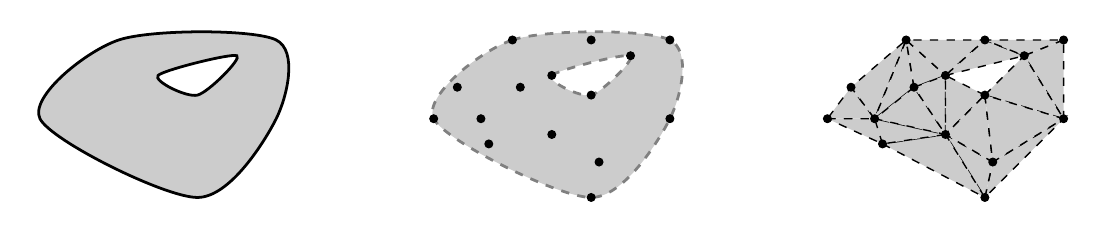
\begin{tikzpicture}
          \draw [black, line width=1, fill=black!20!white] plot [smooth cycle] coordinates {(0,0) (1,1) (3,1) (3,0) (2,-1)};
          \draw [black, line width=1, fill=white] plot [smooth cycle] coordinates {(2.5, 0.8)  (1.5, 0.55) (2, 0.3)     };
      %
      \draw [black!50!white, dashed, line width=1, fill=black!20!white] plot [smooth cycle] coordinates {(5,0) (6,1) (8,1) (8,0) (7,-1)};
          \draw [black!50!white, dashed, line width=1, fill=white] plot [smooth cycle] coordinates {(7, 0.3) (6.5, 0.55) (7.5, 0.8)};
      %
      \draw [black, line width=0.5, fill=black!20!white, circle, dashed  ] (10,0) -- (10.6, 0) -- (10.3, 0.4) -- cycle;
      \draw [black, line width=0.5, fill=black!20!white, circle, dashed  ] (10,0) -- (10.65, 0) -- (10.7, -0.32) -- cycle;
      \draw [black, line width=0.5, fill=black!20!white, circle, dashed  ] (10.6,0) -- (10.3, 0.4) -- (11, 1) -- cycle;
      \draw [black, line width=0.5, fill=black!20!white, circle, dashed  ] (10.6,0) -- (11.1, 0.4) -- (11, 1) -- cycle;
      \draw [black, line width=0.5, fill=black!20!white, circle, dashed  ] (11.5,0.55) -- (11.1, 0.4) -- (11, 1) -- cycle;
      \draw [black, line width=0.5, fill=black!20!white, circle, dashed  ] (11.5,0.55) -- (12, 1) -- (11, 1) -- cycle;
      \draw [black, line width=0.5, fill=black!20!white, circle, dashed  ] (11.5,0.55) -- (12.5, 0.8) -- (12, 1) -- cycle;
      \draw [black, line width=0.5, fill=black!20!white, circle, dashed  ] (13,1) -- (12.5, 0.8) -- (12, 1) -- cycle;
      \draw [black, line width=0.5, fill=black!20!white, circle, dashed  ] (13,1) -- (12.5, 0.8) -- (13, 0) -- cycle;
      \draw [black, line width=0.5, fill=black!20!white, circle, dashed  ] (12,0.3) -- (12.5, 0.8) -- (13, 0) -- cycle;
      \draw [black, line width=0.5, fill=black!20!white, circle, dashed  ] (12,-1) -- (12.1, -0.55) -- (13, 0) -- cycle;
      \draw [black, line width=0.5, fill=black!20!white, circle, dashed  ] (12,-1) -- (12.1, -0.55) -- (11.5, -0.2) -- cycle;
      \draw [black, line width=0.5, fill=black!20!white, circle, dashed  ] (10.7,-0.32) -- (12, -1) -- (11.5, -0.2) -- cycle;
      \draw [black, line width=0.5, fill=black!20!white, circle, dashed  ] (10.7,-0.32) -- (10.6, 0) -- (11.5, -0.2) -- cycle;
      \draw [black, line width=0.5, fill=black!20!white, circle, dashed  ] (11.1, 0.4) -- (10.6, 0) -- (11.5, -0.2) -- cycle;
      \draw [black, line width=0.5, fill=black!20!white, circle, dashed  ] (11.1, 0.4) -- (11.5, 0.55) -- (11.5, -0.2) -- cycle;
      \draw [black, line width=0.5, fill=black!20!white, circle, dashed  ] (12, 0.3) -- (11.5, 0.55) -- (11.5, -0.2) -- cycle;
      \draw [black, line width=0.5, fill=black!20!white, circle, dashed  ] (12, 0.3) -- (12.1, -0.55) -- (11.5, -0.2) -- cycle;
      \draw [black, line width=0.5, fill=black!20!white, circle, dashed  ] (12, 0.3) -- (12.1, -0.55) -- (13, 0) -- cycle;
      %   
      \node [draw=black,fill=black, shape=circle, scale=0.3] at (10, 0) {};
      \node [draw=black,fill=black, shape=circle, scale=0.3] at (11.1, 0.4) {};
      \node [draw=black,fill=black, shape=circle, scale=0.3] at (11.5, 0.55) {};
      \node [draw=black,fill=black, shape=circle, scale=0.3] at (11.5, -0.2) {};
      \node [draw=black,fill=black, shape=circle, scale=0.3] at (12, 0.3) {};
      \node [draw=black,fill=black, shape=circle, scale=0.3] at (12.1, -0.55) {};
      \node [draw=black,fill=black, shape=circle, scale=0.3] at (13, 0) {};
      \node [draw=black,fill=black, shape=circle, scale=0.3] at (10.7, -0.32) {};
      \node [draw=black,fill=black, shape=circle, scale=0.3] at (10.6, 0) {};
      \node [draw=black,fill=black, shape=circle, scale=0.3] at (12, -1) {};
      \node [draw=black,fill=black, shape=circle, scale=0.3] at (12.5, 0.8) {};
      \node [draw=black,fill=black, shape=circle, scale=0.3] at (10.3, 0.4) {};
      \node [draw=black,fill=black, shape=circle, scale=0.3] at (11, 1) {};
      \node [draw=black,fill=black, shape=circle, scale=0.3] at (12, 1) {};
      \node [draw=black,fill=black, shape=circle, scale=0.3] at (13, 1) {};
      %  
      \node [draw=black,fill=black, shape=circle, scale=0.3] at (5, 0) {};
      \node [draw=black,fill=black, shape=circle, scale=0.3] at (6.1, 0.4) {};
      \node [draw=black,fill=black, shape=circle, scale=0.3] at (6.5, 0.55) {};
      \node [draw=black,fill=black, shape=circle, scale=0.3] at (6.5, -0.2) {};
      \node [draw=black,fill=black, shape=circle, scale=0.3] at (7, 0.3) {};
      \node [draw=black,fill=black, shape=circle, scale=0.3] at (7.1, -0.55) {};
      \node [draw=black,fill=black, shape=circle, scale=0.3] at (8, 0) {};
      \node [draw=black,fill=black, shape=circle, scale=0.3] at (5.7, -0.32) {};
      \node [draw=black,fill=black, shape=circle, scale=0.3] at (5.6, 0) {};
      \node [draw=black,fill=black, shape=circle, scale=0.3] at (7, -1) {};
      \node [draw=black,fill=black, shape=circle, scale=0.3] at (7.5, 0.8) {};
      \node [draw=black,fill=black, shape=circle, scale=0.3] at (5.3, 0.4) {};
      \node [draw=black,fill=black, shape=circle, scale=0.3] at (6, 1) {};
      \node [draw=black,fill=black, shape=circle, scale=0.3] at (7, 1) {};
      \node [draw=black,fill=black, shape=circle, scale=0.3] at (8, 1) {};
      %
      
        \end{tikzpicture}
        }
      }
      \caption{Continuous and analogous discrete manifolds with one $1$-dimensional hole ($\dim \bar{\mc H}_1=1$). Left pane: the continuous manifold; center pane: the discretization with mesh vertices; right pane: a simplicial complex built upon the mesh. Triangles in the simplicial complex $\mc K$ are colored gray (right). 
      \label{fig:example_holes}
      }
    \end{figure}
    

Indeed, simplicial complex \( \mc K \) is not a manifold, although it may be seen as a discretization of the manifold, \Cref{fig:example_holes}. Moreover, one can show the convergence of the discrete homology group \( \mc H_k \) to its continuous counterpart in case of \( k = 1 \) in thermodynamic limit, \todo{refs}.



\subsubsection{ Elements of the Hodge decomposition as harmonic/vorticity/potential flow}
      \todo{ Maybe we will need here a quick discussion with connection to the continuous case }

Similarly, simplicial complex-specific case of the Hodge's decomposition, \Cref{thm:hodge_decomposition}, holds:
\begin{equation}
      \ds R^{m_k} = \lefteqn{\overbrace{\phantom{\im B_k^\top \oplus  \ker \left( B_k^\top B_k + B_{k+1} B_{k+1}^\top \right)}}^{\ker B_{k+1}^\top}} \im B_k^\top \oplus
      \underbrace{\ker \left( B_k^\top B_k + B_{k+1} B_{k+1}^\top \right) \oplus  \im B_{k+1}}_{\ker B_k}            
\end{equation}


\begin{definition}[Hodge Laplacian Operator]
      Let \( \mc K \) be a simplicial complex with corresponding boundary maps \( B_k \). Then due to \Cref{thm:two_kernels} and \Cref{lemma:hodge_kernels},
      \begin{equation}
            \mc H_k \cong \ker \left( B_k^\top B_k + B_{k+1} B_{k+1}^\top \right)
      \end{equation}
      Operator \( L_k =  B_k^\top B_k + B_{k+1} B_{k+1}^\top \) is known as \(k\)-th \emph{Hodge Laplacian} (or \emph{higher-order Laplacian}) operator. Two terms \( \Ld k =B_k^\top B_k  \) and \( \Lu k = B_{k+1} B_{k+1}^\top \) are known as \(k\)-th \emph{down}- and \emph{up}-Laplacians respectively.
\end{definition}

As established above, the homology group \( \mc H_k \cong \ker L_k \) consists of \emph{harmonic representative} or \emph{harmonic chains} (which name is explained by the fact of falling into the kernel of the corresponding Laplacian operator \( L_k \)). ELements of the remaining components of the decomposition can be described through the analogy with differential operator on simplicial complexes. For instance, 
\begin{enumerate}
      \item the conjugate boundary map \( B_1^\top \) is a discrete derivative on the graph: \( B_1^\top  [u_1, u_2 ] = [ u_2 ] - [u_1]\), hence \( B_1^\top  = \grad \) and \( B_1 =  -\diver \);
      \item the conjugate boundary map \( B_2^\top \) is a discrete \( \curl \) operator: \( B_2^\top [u_1, u_2, u_3 ] = [u_1, u_2] - [u_1, u_3]+[u_2, u_3] = [u_1, u_2] +[u_2, u_3] + [u_3, u_1]\); note that the fundamental lemma of homology de facto restates a widely known fact \( \curl \grad = 0 \);
      \item \(1\)-st order Hodge Laplacian operator then can be rewritten as a composition of the differential operators:
      \begin{equation}
            L_1 = - \grad \diver + \curl^* \curl = \Delta_1
      \end{equation}
      Operator \( \Delta_1 \) is known as a \emph{Helmholzian operator on graphs}, an analogue of the vector Laplacian, \cite{hanlonLaplacianMethod2002}.
\end{enumerate}

Following this, the elements of \( \im B_1^\top = \im ( \grad )\) are refered as \emph{potential flows} (since each element \( y_i\) of a vector \( \b y = B_1^\top \b x \) is a difference of potentials between some pair nodes \( \alpha \) and \( \beta \) forming the \(i\)-th edge); similarly, elements of \( \im B_2 = \im( \curl^*)\) are \emph{vector potentials} or \emph{vorticities}, and \( \ker B_1 \) and \( \ker B_2^\top \) are divergence- and curl-free flows respectively (a more low level discussion of these two subspaces is provided further).

\begin{remark}
      Consideration above provides a solid intuition but lacks clearly formality: indeed, in order to properly define graph's gradient, divergence and curl operators, one would need to discuss alternating functions on a graph (co-chains) and corresponding coboundary operator and cohomology,~\cite{limHodgeLaplaciansGraphs2020}, and show a direct connection with dicrete differential forms on manifolds. We choose to abstain from the introduction of another quite abstract entity since it should not affect the clarity of the numerical analysis of the Laplacian operators conducted further.
\end{remark}







\subsubsection{ Laplacian operators \( L_k \) }

The \(k\)-th order Hodge Laplacian operator \( L_k = B_k^\top B_k + B_{k+1} B_{k+1}^\top \) naturally joins the boundary relational information about simplices of differents orders in \( \mc K \) and describes the topological structure of the complex.

In its matrix form, \( L_k \) is symmetric ( \( L_k^\top = L_k\) ) and semi-positive definite ( \( \b x^\top L_k \b x = \b x^\top  B_k^\top B_k \b x  + \b x^\top B_{k+1} B_{k+1}^\top \b x = \| B_k \b x \|^2 + \| B_{k+1}^\top \b x \|^2 \ge 0 \) ) operator. Moreover, individual entries of down- and up-Laplacians \( \Ld k \) and \( \Lu k \) describe oriented adjacency of simplices in \( \V k \). Namely, two simplices \( \sigma, \sigma' \in \V k \) are down-adjacent by a common face \( \tau \in \V {k-1}\) with a similar  (so the orientation  of a common face agrees or disagrees with the orientation of \( \sigma \) and \( \sigma' \) simultaneously) and dissimilar orientation (otherwise); analogously, one can define an upper-adjacent pair \( \sigma, \sigma' \in \V k\) belonging to the same \( \tau \in \V {k+1} \). Then
\begin{equation}
      [ \Ld k ]_{ij} = \begin{cases}
            k+1, \qquad \text{if } i = j \\
            \phantom{k+}1, \qquad \text{if } i \ne j  \text{ and } \sigma_i, \sigma_j \text{ are upper-adjacent with similar orienation} \\
            \phantom{k}-1, \qquad \text{if } i \ne j \text{ and } \sigma_i, \sigma_j \text{ are upper-adjacent with dissimilar orienation} \\
            \phantom{k+}0 \qquad \text{otherwise}
      \end{cases}
\end{equation}
\begin{equation}
      [ \Lu k ]_{ij} = \begin{cases}
            \deg(\sigma_i), \qquad \text{if } i = j \\
            \phantom{k+}1, \qquad \text{if } i \ne j  \text{ and } \sigma_i, \sigma_j \text{ are down-adjacent with similar orienation} \\
            \phantom{k}-1, \qquad \text{if } i \ne j \text{ and } \sigma_i, \sigma_j \text{ are down-adjacent with dissimilar orienation} \\
            \phantom{k+}0 \qquad \text{otherwise}
      \end{cases}
\end{equation}
where \( \deg(\sigma_i) \) is the number of simplices in \( \V {k+1}\) having \( \sigma_i\) as a face.

\todo{figure?}

\subsubsection{ Classical Laplacian and its kernel elements }

Homology groups described above are not necessarily devoted to the case of higher-order interaction (or, equally, high order simplicial complexes \( \mc K \)). Indeed, the \( 0 \)-order homology group is properly defined for \( 0\)-skeleton of any simplicial complex, or, in other words, the classical graph.

Assuming the absent boundary of a node, \( B_0 = 0 \), the \( 0 \)-order Hodge Laplacian or classical graph Laplacian \( L_0 \) is defined as
\begin{equation}
      L_0 = B_1 B_1^\top \qquad \text{and} \qquad \mc H_0 = \ker B_1^\top
\end{equation}



 \subsubsection{ Kernel elements of \( L_k \) }

\todo{Some relation to the continuous case}

\paragraph{ Spreading and balancing as a mechanism of the non-local circulation}
















\section{ Weigthed and Normalised Boundary Operators}

\todo{definition and motivation of the weighting scheme}






Note that, from the definition \( \bar B_k= W_{k-1}^{-1} B_k W_k \) and \eqref{eq:Bk_Bk+1_0}, we immediately have that  \( \bar B_k\bar B_{k+1}=0 \). Thus, the group \( \bar {\mc H}_k = \ker \bar B_k / \im \bar B_{k+1} \) is well defined for any choice of positive weights  \( w_k \) and is isomorphic to \( \ker \bar L_k \). While the homology group may depend on the weights,  we observe below that its dimension does not. Precisely, we have 
\begin{proposition}
 \label[proposition]{thm:wHomGroup}
     The dimension of the homology groups of \( \mc K \) is not affected by the weights of its \( k \)-simplicies. Precisely, if \( W_k \) are positive diagonal matrices, we have
     \begin{equation}
         \dim \ker \bar B_k = \dim \ker B_k, \quad \dim \ker \bar B_k^\top = \dim \ker B_k^\top, \quad \dim \bar{\mc H}_k = \dim \mc H_k\, .
     \end{equation}
     Moreover, \( \ker B_k = W_k \ker \bar B_k \) and \( \ker B_k^\top = W_{k-1}^{-1} \ker \bar B_k^\top \).
\end{proposition}

\begin{proof}
Since \( W_k \) is an invertible diagonal matrix, 
\begin{equation*}
    \bar B_k \b x = 0 \iff W_{k-1}^{-1}B_k W_k \vec x =0 \iff B_k W_k \vec x =0. 
\end{equation*}
Hence, if \( \vec x \in \ker \bar B_k \), then \( W_k \vec x \in \ker B_k \), and, since \( W_k \) is bijective, \( \dim \ker \bar B_k = \dim \ker B_k \). Similarly, one observes that \( \dim \ker \bar B_k^\top = \dim \ker B_k^\top \).

Moreover, since \( \bar B_k \bar B_{k+1} =0 \), then \( \im \bar B_{k+1} \subseteq \ker \bar B_k \) and \( \im \bar B_k^\top \subseteq \ker \bar B_{k+1}^\top \). This yields \( \ker \bar B_k \cup \ker \bar B_{k+1}^\top = \mathbb{R}^{\mc V_k} = \ker B_k \cup \ker  B_{k+1}^\top\). Thus, for the homology group it holds:
\begin{equation*}
      \begin{aligned}
    \dim \bar {\mc H}_k & = \dim \left( \ker \bar B_k \cap \ker \bar B_{k+1}^\top \right)= \\
    & = \dim \ker \bar B_k + \dim \ker \bar B_{k+1}^\top - \dim \left( \ker \bar B_k \cup \ker \bar B_{k+1}^\top \right) = \\
    & = \dim \ker B_k + \dim \ker  B_{k+1}^\top - \dim \left( \ker  B_k \cup \ker  B_{k+1}^\top \right) = \dim \mc H_k
      \end{aligned}
\end{equation*}
\end{proof}


\todo{normalisation theorem}



\section{Matrix nearness problems}



\subsection{ 101 on MNP }

Generally speaking, for a given matrix \( A \) a \emph{matrix nearness problem} consists of finding the closest possible matrix \( X \) among the admissible set with a number of desired properties. For instance, one may search for the closest (in some metric) symmetric positive/negative definite matrix, unitary matrix or the closest graph Laplacian. 

Motivated by the topological meaning of the \emph{kernel} of Hodge Laplacians \( L_k \), we assume the specific case of \emph{spectral} MNPs: here one aims for the target matrix \( X \) to have a specific spectrum \( \sigma(X) \). For instance in the stability study of the dynamical system \( \dot{\b x} = A \b x \) one can search for the closest Hurwitz matrix such that \( \mathrm{Re} \left[ \lambda_i \right] < 0 \) for all \( \lambda_i \in \sigma(X) \); similarly, assuming given matrix \( A \) is a graph Laplacian, one can search for the closest disconnected graph (so the algebraic connectivity \( \lambda_2 = 0 \)).

Here we recite the optimization framework developed by REFREFREF\todo{fix it} for the class of the spectral matrix nearness problems; one should note, however, that this is by far not the only approach to the task, REFREFREF\todo{also fix it with Nicholas and others, I guess?}.

\paragraph{Functional and Gradient Flow}

Let as assume that \( X = A + \Delta \) and intead of searching for \( X \), we search for the perturbation matrix \( \Delta \); additionally, we assume that \( \Omega \) is the admissible set containing all possible perturbations \( \Delta \).
















\subsection{Direct approach: failure and discontinuity problems }


\subsubsection{Principal spectral inheritance}


Before moving on to the next section, we recall here a relatively direct  but important spectral property that connects the spectra of the $k$-th and $(k+1)$-th order Laplacians. 

\begin{theorem}[HOL's spectral inheritance]\label{thm:inherit}
  Let $L_k$ and $L_{k+1}$ be  higher-order Laplacians for the same simplicial complex $\mc K$. Let $\bar L_k=\bar L_k^{down}+\bar L_k^{up}$, where $\bar L_k^{down}=\bar B_k^\top \bar B_k$ and $\bar L_k^{up}=\bar B_{k+1} \bar B_{k+1}^\top$. Then:
  \begin{enumerate}
    \item $\sigma_+(\bar L_k^{up})=\sigma_+(\bar L_{k+1}^{down})$, where $\sigma_+(\cdot)$ denotes the positive part of the spectrum;
    \item if $ 0 \ne \mu \in \sigma_+(\bar L_k^{up}) = \sigma_+(\bar L_{k+1}^{down})$, then the eigenvectors are related as follows:
    \begin{enumerate}
      \item if $\vec x$ is and eigenvector for $\bar L_k^{up}$ with the eigenvalue $\mu$, then $\vec y = \frac{1}{\sqrt{\mu}} \bar B_{k+1}^\top \vec x$ is an eigenvector for $\bar L_{k+1}^{down}$ with the same eigenvalue;
      \item if $\vec u$ is and eigenvector for $\bar L_{k+1}^{down}$ with the eigenvalue $\mu$ and $\vec u \notin \ker \bar B_{k+1}$, then $\vec v = \frac{1}{\sqrt{\mu}} \bar B_{k+1} \vec u$ is an eigenvector for $\bar L_{k}^{up}$ with the same eigenvalue;
    \end{enumerate}
    \item for each Laplacian $\bar L_k$: if $\vec v \notin \ker \bar L_k^{down}$ is the eigenvector for $\bar L_k^{down}$, then $\vec v \in \ker \bar L_{k}^{up}$; vice versa, if $\vec u \notin \ker \bar L_k^{up}$ is the eigenvector for $\bar L_k^{up}$, then $\vec v \in \ker \bar L_k^{down}$;
    \item consequently, there exist $\mu \in \sigma_+(\bar L_k)$ with an eigenvector $\vec u \in \ker \bar L_k^{up}$, and $\nu \in \sigma_+(\bar L_{k+1})$ with an eigenvector $\vec u \in \ker \bar L_{k+1}^{down}$, such that:
    $$
    \bar B_k^\top \bar B_k \vec v  = \mu \vec v, \qquad \bar B_{k+2} \bar B_{k+2}^\top \vec u = \nu \vec u\, . 
    $$
  \end{enumerate}
\end{theorem}
\begin{proof}
For $(2a)$ it is sufficient to note that $ \bar L_{k+1}^{down} \vec y = \bar B_{k+1}^\top \bar B_{k+1} \frac{1}{\sqrt{\mu}} \bar B_{k+1}^\top \vec x = \frac{1}{\sqrt{\mu}}\bar B_{k+1}^\top \bar L_k^{up} \vec x = \sqrt \mu \bar B_{k+1}^\top \vec x  = \mu \vec y$. Similarly, for $(2b)$: $\bar L_k^{up} \vec v= \bar B_{k+1} \bar B_{k+1}^\top \frac{1}{\sqrt{\mu}} \bar B_{k+1} \vec u = \frac{1}{\sqrt{\mu}} \bar B_{k+1} \bar L_{k+1}^{down} \vec u = \mu \vec v $; joint $2(a)$ and $2(b)$ yield $(1)$. \emph{Hodge decomposition} immediately yields the strict separation of eigenvectors between $\bar L_k^{up}$ and $\bar L_k^{down}$, $(3)$; given $(3)$, all the inherited  eigenvectors from $(2a)$ fall into the $\ker \bar L_{k+1}^{down}$, thus resulting into $(4)$.
\end{proof}
In other words, the variation of the spectrum of the $k$-th Laplacian when moving from one order to the next one works as follows: 
the down-term $\bar L_{k+1}^{down}$ inherits the positive part of the spectrum from the up-term of  $\bar L_k^{up}$; the  eigenvectors corresponding to the inherited positive part of the spectrum lie in the kernel of $\bar L_{k+1}^{up}$; at the same time, the ``new'' up-term $\bar L_{k+1}^{up}$ has a new, non-inherited, part of the positive spectrum (which, in turn, lies in the kernel of the $(k+2)$-th down-term).

In particular, we notice that for $k = 0$, since $B_0=0$ and $\bar L_0=\bar L_0^{up}$, the  theorem yields $\sigma_+ (\bar L_0 ) = \sigma_+ (\bar{L_1}^{down}) \subseteq \sigma_+(\bar L_1)$. In other terms, the positive spectrum of the $\bar L_0$ is inherited by the spectrum of $\bar L_1$ and the remaining (non-inherited) part of $\sigma_+(\bar L_1)$ coincides with $\sigma_+(\bar L_1^{up})$. 
\Cref{fig:thm_spct_ill} provides an  illustration of the statement of  \Cref{thm:inherit} for $k = 0$.
  \begin{figure}[t]
    \centering
    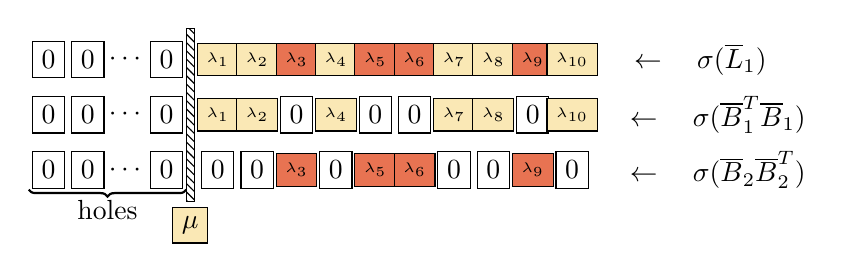
\begin{tikzpicture}
      \node[draw] at (0,0) {0};
      \node[draw] at (0.5,0) {0};
      \node at (1, 0) {$\cdots$};
      \node[draw] at (1.5,0) {0};
      \node[draw, fill=bananamania] at (2.15,0) {\tiny{$\lambda_1$}};
      \node[draw, fill=bananamania] at (2.65,0) {\tiny{$\lambda_2$}};
      \node[draw, fill=burntsienna] at (3.15,0) {\tiny{$\lambda_3$}};
      \node[draw, fill=bananamania] at (3.65,0) {\tiny{$\lambda_4$}};
      \node[draw, fill=burntsienna] at (4.15,0) {\tiny{$\lambda_5$}};
      \node[draw, fill=burntsienna] at (4.65,0) {\tiny{$\lambda_6$}};
      \node[draw, fill=bananamania] at (5.15,0) {\tiny{$\lambda_7$}};
      \node[draw, fill=bananamania] at (5.65,0) {\tiny{$\lambda_8$}};
      \node[draw, fill=burntsienna] at (6.15,0) {\tiny{$\lambda_9$}};
      \node[draw, fill=bananamania] at (6.65,0) {\tiny{$\lambda_{10}$}};
      \node at (8.5, 0) {$\leftarrow \quad \sigma (\bar L_1)$\phantom{$\bar B_1$}};
    
      \node[draw] at (0,-0.7) {0};
      \node[draw] at (0.5,-0.7) {0};
      \node at (1, -0.7) {$\cdots$};
      \node[draw] at (1.5,-0.7) {0};
      \node[draw, fill=bananamania] at (2.15,-0.7) {\tiny{$\lambda_1$}};
      \node[draw, fill=bananamania] at (2.65,-0.7) {\tiny{$\lambda_2$}};
      \node[draw] at (3.15,-0.7) {0};
      \node[draw, fill=bananamania] at (3.65,-0.7) {\tiny{$\lambda_4$}};
      \node[draw] at (4.15,-0.7) {0};
      \node[draw] at (4.65,-0.7) {0};
      \node[draw, fill=bananamania] at (5.15,-0.7) {\tiny{$\lambda_7$}};
      \node[draw, fill=bananamania] at (5.65,-0.7) {\tiny{$\lambda_8$}};
      \node[draw] at (6.15,-0.7) {0};
      \node[draw, fill=bananamania] at (6.65,-0.7) {\tiny{$\lambda_{10}$}};
      \node at (8.5, -0.7) {$\leftarrow \quad \sigma (\bar B_1^T \bar B_1)$};
    
      \node[draw] at (0,-1.4) {0};
      \node[draw] at (0.5,-1.4) {0};
      \node at (1, -1.4) {$\cdots$};
      \node[draw] at (1.5,-1.4) {0};
      \node[draw] at (2.15,-1.4) {0};
      \node[draw] at (2.65,-1.4) {0};
      \node[draw, fill=burntsienna] at (3.15,-1.4) {\tiny{$\lambda_3$}};
      \node[draw] at (3.65,-1.4) {0};
      \node[draw, fill=burntsienna] at (4.15,-1.4) {\tiny{$\lambda_5$}};
      \node[draw, fill=burntsienna] at (4.65,-1.4) {\tiny{$\lambda_6$}};
      \node[draw] at (5.15,-1.4) {0};
      \node[draw] at (5.65,-1.4) {0};
      \node[draw, fill=burntsienna] at (6.15,-1.4) {\tiny{$\lambda_9$}};
      \node[draw] at (6.65,-1.4) {0};
      \node at (8.5, -1.4) {$\leftarrow \quad \sigma (\bar B_2 \bar B_2^T)$};
    
      \draw [
        thick,
        decoration={
            brace,
            mirror,
            raise=0.25cm
        },
        decorate
      ] (-0.25, -1.4) -- (1.75, -1.4) 
    node [pos=0.5,anchor=north,yshift=-0.25cm] {holes}; 
      \draw[pattern=north west lines] (1.75,0.4) rectangle (1.85, -1.8);
      \node[draw, align=center, fill=bananamania] at (1.8,-2.1) {$\mu$};
    \end{tikzpicture}
    \caption{Illustration for the principal spectrum inheritance (\Cref{thm:inherit}) in case $k=0$: spectra of $\bar L_1$, $\bar L_1^{down}$ and $\bar L_1^{up}$ are shown. Colors signify the splitting of the spectrum, $\lambda_i>0 \in \sigma(\bar L_1)$ ; all yellow eigenvalues are inherited from $\sigma_+(\bar L_0)$; red eigenvalues belong to the non-inherited part. Dashed barrier $\mu$ signifies the penalization threshold (see the target functional in \Cref{subsec:functional}) preventing homological pollution (see \Cref{subsec:connetedness}). }
    \label{fig:thm_spct_ill}
    \vspace{-10pt}
  \end{figure}

























%Let \( A \) be a square matrix, \( A \ in \ds C^{n \times n }\); \todo{do we need that?} let \( \lambda ( A )\) be a chosen eigenvalue of the matrix \( A \). For instance, \( \lambda \) can be the eigenvalue with highest/lowest magnitude or real part on the complex plane.

%Generally speaking, \emph{a spectral matrix nearness problem} focuses on finding a matrix \( X \) closest to \( A \) such that the spectrum \( \sigma ( X ) \) satisfies some property. For instance, one can search for the closest matrix such that the rightmost eigenvalue has a zero real part on the complex plane (in the stability study of the continuous dynamical systems) or all the eigenvalues fit on the unit disk (in the stability study of the discrete dynamical systems), etc.

%Let \( \Delta = X - A \); then one aims to find a perturbation \( \Delta \) with a minimal norm, \( \min \| \Delta \| \). Additionally, 
\section{Topological Stability of Simplicial Complexes}
\chapter{Preconditioning}

\todo{
      Here we need to say general words about how we need an efficient preconditioning scheme.
}

\section{Preconditioning 101}

\subsection{ why do we care about the condition number?}


\subsection{ Iterative methods }


\subsection{ CG and convergence  }
      \todo{ CGLS }


\subsection{ Zoo of preconditioners }

      \todo{ Reinforced diagonal} 

      \todo{ Cholesky }
      \todo{ Incomplete Cholesky }


\section{ LSq problem for the whole Laplacian -> up-Laplacian }
      
\section{ Preconditioning on the up-Laplacian }
      
\subsection{ Sparsification (Spielman/Osting) }
      
\subsection{ Cholesky preconditioning for classical graphs  }


\subsubsection{ Stochastic Cholesky preconditioning  }
      
\subsubsection{ Schur complements }


\subsection{ Problem with Schur complements in the case of \( L_1 \)  }

      \todo{  Transition to collapsibility }
      




\section{Collapsible simplicial complexes}

% TODO: introduction

\subsection{ Classical collapsiblity }


In this section we borrow the terminology from \cite{whiteheadSimplicialSpacesNuclei1939}; additionally, let us  assume that considered simplicial complex \( \mc K \) is restricted to its \(2\)-skeleton, so \( \mc K \) consists only of nodes, edges, and triangles, \( \mc K = \V 0 \cup \V 1 \cup \V 2\).

Simplex \( \tau \in \mc K \) is called an (inlusion-wise) {maximal face} of simplex \( \sigma \in \mc K \) if \( \tau \) is maximal by inlusion simplex such that \( \sigma \subseteq \tau \) and \( \ord \sigma < \ord \tau \). 
\begin{figure}[hbtp]
      \centering
      \begin{tikzpicture}

      \fill [opacity=0.5,liberty]    (0, 0) -- (2, 0) --  (1, 1.5) -- cycle;
      \fill [opacity=0.3,liberty]    (0, 0) -- (2, 0) --  (1, -1.5) -- cycle;

      \Vertex[x=0, y=0, style={color=persimmon}, fontcolor=white, size=0.2, label = 1]{v1}
      \Vertex[x=2, y=0, style={color=persimmon}, fontcolor=white, size=0.2, label = 2]{v2}
      \Vertex[x=1, y=1.5, style={color=persimmon}, fontcolor=white, size=0.2, label = 3]{v3}
      \Vertex[x=1, y=-1.5, style={color=persimmon}, fontcolor=white, size=0.2, label = 4]{v4}

      \Edge[](v1)(v2)
      \Edge[](v1)(v3)
      \Edge[](v2)(v3)
      \Edge[](v1)(v4)
      \Edge[](v2)(v4)


\end{tikzpicture}
      \caption{Example of a simplicial complex: free simplices and maximal faces. \label{fig:adjacent_triangles}}
\end{figure}
 For instance, in \Cref{fig:adjacent_triangles} the edge \( \{1, 2\} \) and nodes \( \{ 1 \} \) and \( \{ 2 \} \) have two maximal faces, \( \{ 1, 2, 3 \} \) and \( \{ 1, 2, 4 \} \), while all the other edges and nodes have unique maximal faces --- their corresponding triangles. Note that in the case of the node \( \{ 1 \} \), there are bigger simplices containing it besides the triangles (e.g. the edge \( \{ 1, 2 \} \)), but they are not maximal by inclusion.

\begin{definition}[Free simplex]\label{def:free}
      The simplex \(\sigma \in \mc K \) is {free} if it has exactly one maximal face \( \tau \), \( \tau = \tau(\sigma) \). F.i. edges \( \{ 1, 3 \} \), \( \{ 1, 4 \} \), \( \{ 2, 3 \} \) and \( \{ 2, 4 \} \) are all free in \Cref{fig:adjacent_triangles}.
\end{definition} 

 The {collapse} \( \mc K \backslash \{ \sigma \} \) of \( \mc K \) at a free simplex \( \sigma \) is the transition from the original simplicial complex \( \mc K \) to a smaller simplicial complex \( \mc L \) without the free simplex \( \sigma \) and the corresponding maximal face \( \tau \), \( \mc K \to \mc K' = \mc K - \sigma - \tau \); namely, one can eliminate a simplex \( \tau \) if it has an accessible (not included in another simplex) face \(\sigma\).

Naturally, one can perform several consequent collapses at  \( \Sigma = \{ \sigma_1, \sigma_2, \ldots \} \) assuming \( \sigma_i \) is free in collapse simplicial complex from the previous stage; \( \Sigma \) is called the {collapsing sequence}. Formally:
 \begin{definition}[Collapsing sequence]
       Let \( \mc K \) be a simplicial complex. \( \Sigma = \{ \sigma_1, \sigma_2, \ldots \} \) is a {collapsing sequence} if \( \sigma_1 \) is free in \( \mc K \) and each \( \sigma_i \), \( i > 1 \), is free at 
       \( \mc K^{(i)} = \mc K^{(i-1)} \backslash \{ \sigma_i \} \), \( \mc K^{(1)} = \mc K \). The collapse of \( \mc K \) to a new complex \( \mc L \) at \( \Sigma \) is denoted by \( \mc L = \mc K \backslash \Sigma \).
 \end{definition}
 By the definition, every collapsing sequence \( \Sigma \) has a corresponding sequence \( \ds T = \{ \tau(\sigma_1), \tau(\sigma_2), \ldots \} \) of maximal faces being collapsed at every step.

 \begin{definition}[Collapsible simplicial complex, \cite{whiteheadSimplicialSpacesNuclei1939}]
      The simplicial complex \( \mc K \) is {collapsible} if there exists a collapsing sequence \( \Sigma \) such that \( \mc K \) collapses to a single vertex at \( \Sigma \), \( \mc K \backslash \Sigma = \{ v \} \).
\end{definition}

Determining whether the complex is collapsible is in general \emph{NP-complete},~\cite{tancerRecognitionCollapsibleComplexes2016}, but can be almost linear for a set of specific families of \( \mc K \), e.g.\ if the simplex can be embeded into the triangulation of the \(d\)-dimensional unit sphere,~\cite{cohenSolving1laplaciansNearly2014}. Naturally restricting the collapses to the case of \(d\)-collapses (such that \( \ord \sigma_i \le d-1 \)), one arrive at the notion of \(d\)-collapsibility,~\cite{tancerDcollapsibilityNPcomplete2009}.

\begin{definition}[\(d\)-Core]
      A \(d\)-Core is a subcomplex of \( \mc K \) such that every simplex of order \( d - 1\) belongs to at least \( 2 \) simplices of order \( d \). E.g. \(2\)-Core is such a subcomplex of the original 2-skeleton \( \mc K \) that every edge from \( \V 1 \) belong to at least \(2\) triangles from \( \V 2 \).
\end{definition}

\begin{lemma}[\cite{lofanoWorstWayCollapse2021}]
      \( \mc K \) is \(d\)-collapsible if and only if it does not contain a \( d\)-core.
\end{lemma}
\begin{proof}
      The proof of the lemma above naturally follows from the definition of the core. Assume \( \Sigma \) is a \(d\)-collapsing sequence, and \( \mc K \backslash \Sigma \) consists of more than a single vertex and has no free simplices of order \( \le d-1\) (``collapsing sequence gets stuck''). Then, each simplex of order \( d-1 \) is no free but belongs to at least \(2\) simplices of order \(d\), so \( \mc K \backslash \Sigma \) is a \( d \)-Core. 
      
      Conversely if a \(d\)-Core exists in the complex, the collapsing sequence should necessarily include its simplices of order \( d - 1 \) which can not become free during as a result of a sequence of collapses. Indeed, for \(\sigma\) from \(d\)-Core,  \(\ord \sigma = d-1\), to become free, one needs to collapse at least one of \(\sigma\)'s maximal faces for \( d\)-Core , all of whose faces are, in turn, contained in the \( d\)-Core (since \(d\)-Core is a simplicial complex). As a result one necessarily needs a prior collapse inside the \(d\)-Core to perform the first collapse in the \(d\)-Core, which is impossible.
\end{proof}

In the case of the classical graph model, the \( 1 \)-Core is a subgraph where each vertex has a degree at least \( 2 \); in other words, \( 1 \)-Core cannot be a tree and necessarily contains a simple cycle. Hence, the collapsibility of a classical graph coincides with the acyclicity. The \(d\)-Core is the generalization of the cycle for the case of \(1\)-collapsibility of the classical graph; additionally, the \(d\)-Core is very dense due to its definition. In the case of \(2\)-Core, we provide simple exemplary structures on \Cref{fig:2-core} which imply various possible configurations for a  \(d\)-Core, \( d \ge 2 \), hence a search for \(d\)-Core inside \( \mc K \) is neither trivial, no computationally cheap.

\begin{figure}[htbp]
      \centering
      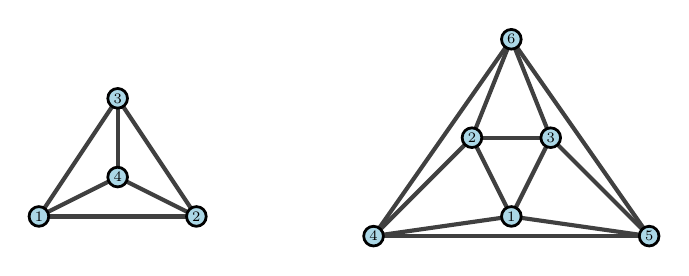
\begin{tikzpicture}
      \Vertex[x=0, y=0, size=0.25, fontscale=0.75, label=1]{v1}
      \Vertex[x=2, y=0, size=0.25, fontscale=0.75,label=2]{v2}
      \Vertex[x=1, y=1.5, size=0.25,fontscale=0.75, label=3]{v3}
      \Vertex[x=1, y=0.5, size=0.25,fontscale=0.75, label=4]{v4} 
      \Edge(v1)(v2)
      \Edge(v1)(v3)
      \Edge(v1)(v4)
      \Edge(v2)(v3)
      \Edge(v2)(v4)
      \Edge(v3)(v4)

      
      \Vertex[x=6, y=0, size=0.25, fontscale=0.75, label=1]{v1}
      \Vertex[x=5.5, y=1, size=0.25, fontscale=0.75, label=2]{v2}
      \Vertex[x=6.5, y=1, size=0.25, fontscale=0.75, label=3]{v3}
      \Vertex[x=4.25, y=-0.25, size=0.25, fontscale=0.75, label=4]{v4}
      \Vertex[x=7.75, y=-0.25, size=0.25, fontscale=0.75, label=5]{v5}
      \Vertex[x=6, y=2.25, size=0.25, fontscale=0.75, label=6]{v6}
      \Edge(v1)(v2)
      \Edge(v2)(v3)
      \Edge(v1)(v3)
      \Edge(v4)(v5)
      \Edge(v4)(v6)
      \Edge(v5)(v6)
      \Edge(v1)(v4)
      \Edge(v1)(v5)
      \Edge(v2)(v6)
      \Edge(v3)(v6)
      \Edge(v2)(v4)
      \Edge(v3)(v5)
\end{tikzpicture}
      \caption{ \(2\)-Core, examples. \label{fig:2-core} }
\end{figure}

%Besides the quantitative restriction discussed later, \( 2 \)-Cores tend to appear relatively early when upon ``densifying'' the complex.
Additionally, we demonstrate that an arbitrary simplicial complex \(\mc K\) tends to contain \(2\)-Cores as long as \( \mc K \) is denser than a trivially collapsible case. Assume the complex formed by triangulation of \( m_0 \) random points on the unit square with a sparsity pattern \( \nu \); the triangulation itself with the corresponding \( \nu_\Delta \) is collapsible, but a reasonably small addition of edges already creates a \(2\)-Core (since it is local), \Cref{fig:core_prob}, left. Similarly, sampled sensor networks, where \( \exists \sigma \in \V 1: \; \sigma = [v_1, v_2] \iff \| v_1 - v_2 \|_2 < \eps \) for a chosen percolation parameter \( \eps > 0 \), quickly form a 2-Core upon the densifying of the network.

\begin{figure}[htbp]
      \centering
      \scalebox{0.4}{
            % Recommended preamble:
% \usetikzlibrary{arrows.meta}
% \usetikzlibrary{backgrounds}
% \usepgfplotslibrary{patchplots}
% \usepgfplotslibrary{fillbetween}
% \pgfplotsset{%
%     layers/standard/.define layer set={%
%         background,axis background,axis grid,axis ticks,axis lines,axis tick labels,pre main,main,axis descriptions,axis foreground%
%     }{
%         grid style={/pgfplots/on layer=axis grid},%
%         tick style={/pgfplots/on layer=axis ticks},%
%         axis line style={/pgfplots/on layer=axis lines},%
%         label style={/pgfplots/on layer=axis descriptions},%
%         legend style={/pgfplots/on layer=axis descriptions},%
%         title style={/pgfplots/on layer=axis descriptions},%
%         colorbar style={/pgfplots/on layer=axis descriptions},%
%         ticklabel style={/pgfplots/on layer=axis tick labels},%
%         axis background@ style={/pgfplots/on layer=axis background},%
%         3d box foreground style={/pgfplots/on layer=axis foreground},%
%     },
% }

\begin{tikzpicture}[/tikz/background rectangle/.style={fill={rgb,1:red,1.0;green,1.0;blue,1.0}, draw opacity={1.0}}, show background rectangle]
      \begin{axis}[point meta max={nan}, point meta min={nan}, legend cell align={left}, legend columns={1}, title={}, title style={at={{(0.5,1)}}, anchor={south}, font={{\fontsize{18 pt}{23.400000000000002 pt}\selectfont}}, color={rgb,1:red,0.0;green,0.0;blue,0.0}, draw opacity={1.0}, rotate={0.0}, align={center}}, legend style={color={rgb,1:red,0.1333;green,0.1333;blue,0.3333}, draw opacity={0.1}, line width={1}, solid, fill={rgb,1:red,1.0;green,1.0;blue,1.0}, fill opacity={0.9}, text opacity={1.0}, font={{\fontsize{22 pt}{28.6 pt}\selectfont}}, text={rgb,1:red,0.0;green,0.0;blue,0.0}, cells={anchor={center}}, at={(0.98, 0.02)}, anchor={south east}}, axis background/.style={fill={rgb,1:red,1.0;green,1.0;blue,1.0}, opacity={1.0}}, anchor={north west}, xshift={1.0mm}, yshift={-1.0mm}, width={150.4mm}, height={150.4mm}, scaled x ticks={false}, xlabel={$\mathrm{sparsity \; (wrt \; triangulation)}$}, x tick style={draw={none}}, x tick label style={color={rgb,1:red,0.0;green,0.0;blue,0.0}, opacity={1.0}, rotate={0}}, xlabel style={at={(ticklabel cs:0.5)}, anchor=near ticklabel, at={{(ticklabel cs:0.5)}}, anchor={near ticklabel}, font={{\fontsize{22 pt}{28.6 pt}\selectfont}}, color={rgb,1:red,0.0;green,0.0;blue,0.0}, draw opacity={1.0}, rotate={0.0}}, xmode={log}, log basis x={10}, xmajorgrids={true}, xmin={0.993342357875681}, xmax={1.2577738078862484}, xticklabels={{$\nu_\Delta$,$1.1\nu_\Delta$,$1.25\nu_\Delta$}}, xtick={{1.0,1.1,1.25}}, xtick align={inside}, xticklabel style={font={{\fontsize{18 pt}{23.400000000000002 pt}\selectfont}}, color={rgb,1:red,0.0;green,0.0;blue,0.0}, draw opacity={1.0}, rotate={0.0}}, x grid style={color={rgb,1:red,0.1333;green,0.1333;blue,0.3333}, draw opacity={0.1}, line width={0.5}, solid}, extra x ticks={{}}, extra x tick labels={}, extra x tick style={grid={major}, x grid style={color={rgb,1:red,0.1333;green,0.1333;blue,0.3333}, draw opacity={0.05}, line width={0.5}, solid}, major tick length={0}}, x axis line style={{draw opacity = 0}}, scaled y ticks={false}, ylabel={$\mathrm{probability \; of \; 2-Core}$}, y tick style={draw={none}}, y tick label style={color={rgb,1:red,0.0;green,0.0;blue,0.0}, opacity={1.0}, rotate={0}}, ylabel style={at={(ticklabel cs:0.5)}, anchor=near ticklabel, at={{(ticklabel cs:0.5)}}, anchor={near ticklabel}, font={{\fontsize{22 pt}{28.6 pt}\selectfont}}, color={rgb,1:red,0.0;green,0.0;blue,0.0}, draw opacity={1.0}, rotate={0.0}}, ymode={log}, log basis y={10}, ymajorgrids={true}, ymin={0.23981602983131609}, ymax={1.0424657608411214}, yticklabels={{$0.25$,$0.5$,$1$}}, ytick={{0.25,0.5,1.0}}, ytick align={inside}, yticklabel style={font={{\fontsize{18 pt}{23.400000000000002 pt}\selectfont}}, color={rgb,1:red,0.0;green,0.0;blue,0.0}, draw opacity={1.0}, rotate={0.0}}, y grid style={color={rgb,1:red,0.1333;green,0.1333;blue,0.3333}, draw opacity={0.1}, line width={0.5}, solid}, extra y ticks={{}}, extra y tick labels={}, extra y tick style={grid={major}, y grid style={color={rgb,1:red,0.1333;green,0.1333;blue,0.3333}, draw opacity={0.05}, line width={0.5}, solid}, major tick length={0}}, y axis line style={{draw opacity = 0}}, colorbar={false}]
          \addplot[color={rgb,1:red,0.8;green,0.4;blue,0.4667}, name path={393a1deb-0ad5-49fa-841c-c2d680cf69bc}, draw opacity={1.0}, line width={1.2}, solid, mark={*}, mark size={4.5 pt}, mark repeat={1}, mark options={color={rgb,1:red,0.0;green,0.0;blue,0.0}, draw opacity={1.0}, fill={rgb,1:red,0.8;green,0.4;blue,0.4667}, fill opacity={1.0}, line width={0.0}, rotate={0}, solid}]
              table[row sep={\\}]
              {
                  \\
                  1.009246153846154  0.25  \\
                  1.0134923076923077  0.25  \\
                  1.0177384615384615  0.25  \\
                  1.0219846153846153  0.25  \\
                  1.0262307692307693  0.41  \\
                  1.030476923076923  0.41  \\
                  1.0347230769230769  0.41  \\
                  1.0389692307692306  0.558  \\
                  1.0432153846153847  0.558  \\
                  1.0474615384615384  0.558  \\
                  1.0517076923076922  0.558  \\
                  1.0559538461538462  0.674  \\
                  1.0602  0.674  \\
                  1.0644461538461538  0.674  \\
                  1.0686923076923076  0.674  \\
                  1.0729384615384616  0.758  \\
                  1.0771846153846154  0.758  \\
                  1.0814307692307692  0.758  \\
                  1.0856769230769232  0.846  \\
                  1.089923076923077  0.846  \\
                  1.0941692307692308  0.846  \\
                  1.0984153846153846  0.846  \\
                  1.1026615384615386  0.898  \\
                  1.1069076923076924  0.898  \\
                  1.1111538461538462  0.898  \\
                  1.1154  0.94  \\
                  1.119646153846154  0.94  \\
                  1.1238923076923077  0.94  \\
                  1.1281384615384615  0.94  \\
                  1.1323846153846155  0.958  \\
                  1.1366307692307693  0.958  \\
                  1.1408769230769231  0.958  \\
                  1.145123076923077  0.958  \\
                  1.149369230769231  0.974  \\
                  1.1536153846153847  0.974  \\
                  1.1578615384615385  0.974  \\
                  1.162107692307692  0.988  \\
                  1.166353846153846  0.988  \\
                  1.1705999999999999  0.988  \\
                  1.1748461538461537  0.988  \\
                  1.1790923076923077  0.994  \\
                  1.1833384615384615  0.994  \\
                  1.1875846153846152  0.994  \\
                  1.191830769230769  0.994  \\
                  1.196076923076923  0.998  \\
                  1.2003230769230768  0.998  \\
                  1.2045692307692306  0.998  \\
                  1.2088153846153846  1.0  \\
                  1.2130615384615384  1.0  \\
                  1.2173076923076922  1.0  \\
                  1.221553846153846  1.0  \\
                  1.2258  1.0  \\
                  1.2300461538461538  1.0  \\
                  1.2342923076923076  1.0  \\
                  1.2385384615384614  1.0  \\
                  1.2427846153846154  1.0  \\
                  1.2470307692307692  1.0  \\
              }
              ;
          \addlegendentry {$\mathcal{V}_0(\mathcal K)=24$}
          \addplot[color={rgb,1:red,0.2;green,0.1333;blue,0.5333}, name path={3388d577-df0a-4b0f-bb98-8e4a3883b6b4}, draw opacity={1.0}, line width={1.2}, solid, mark={*}, mark size={4.5 pt}, mark repeat={1}, mark options={color={rgb,1:red,0.0;green,0.0;blue,0.0}, draw opacity={1.0}, fill={rgb,1:red,0.2;green,0.1333;blue,0.5333}, fill opacity={1.0}, line width={0.0}, rotate={0}, solid}]
              table[row sep={\\}]
              {
                  \\
                  1.0153999999999999  0.476  \\
                  1.0179999999999998  0.476  \\
                  1.0206  0.476  \\
                  1.0231999999999999  0.476  \\
                  1.0257999999999998  0.476  \\
                  1.0283999999999998  0.476  \\
                  1.031  0.476  \\
                  1.0335999999999999  0.476  \\
                  1.0361999999999998  0.476  \\
                  1.0388  0.476  \\
                  1.0413999999999999  0.476  \\
                  1.0439999999999998  0.8  \\
                  1.0466  0.8  \\
                  1.0492  0.8  \\
                  1.0517999999999998  0.8  \\
                  1.0543999999999998  0.8  \\
                  1.057  0.8  \\
                  1.0595999999999999  0.8  \\
                  1.0621999999999998  0.8  \\
                  1.0648  0.8  \\
                  1.0674  0.8  \\
                  1.0699999999999998  0.8  \\
                  1.0726  0.916  \\
                  1.0752  0.916  \\
                  1.0777999999999999  0.916  \\
                  1.0803999999999998  0.916  \\
                  1.083  0.916  \\
                  1.0856  0.916  \\
                  1.0881999999999998  0.916  \\
                  1.0908  0.916  \\
                  1.0934  0.916  \\
                  1.0959999999999999  0.916  \\
                  1.0986  0.916  \\
                  1.1011999999999997  0.972  \\
                  1.1037999999999997  0.972  \\
                  1.1063999999999998  0.972  \\
                  1.1089999999999998  0.972  \\
                  1.1115999999999997  0.972  \\
                  1.1141999999999999  0.972  \\
                  1.1167999999999998  0.972  \\
                  1.1193999999999997  0.972  \\
                  1.1219999999999999  0.972  \\
                  1.1245999999999998  0.972  \\
                  1.1271999999999998  0.972  \\
                  1.1297999999999997  0.986  \\
                  1.1323999999999999  0.986  \\
                  1.1349999999999998  0.986  \\
                  1.1375999999999997  0.986  \\
                  1.1401999999999999  0.986  \\
                  1.1427999999999998  0.986  \\
                  1.1453999999999998  0.986  \\
                  1.148  0.986  \\
                  1.1505999999999998  0.986  \\
                  1.1531999999999998  0.986  \\
                  1.1557999999999997  0.986  \\
                  1.1583999999999999  0.998  \\
                  1.1609999999999998  0.998  \\
                  1.1635999999999997  0.998  \\
                  1.1662  0.998  \\
                  1.1687999999999998  0.998  \\
                  1.1713999999999998  0.998  \\
                  1.174  0.998  \\
                  1.1765999999999999  0.998  \\
                  1.1791999999999998  0.998  \\
                  1.1817999999999997  0.998  \\
                  1.1844  0.998  \\
                  1.1869999999999998  1.0  \\
                  1.1895999999999998  1.0  \\
                  1.1922  1.0  \\
                  1.1947999999999999  1.0  \\
                  1.1973999999999998  1.0  \\
                  1.2  1.0  \\
                  1.2026  1.0  \\
                  1.2051999999999998  1.0  \\
                  1.2077999999999998  1.0  \\
                  1.2104  1.0  \\
                  1.2129999999999999  1.0  \\
                  1.2155999999999998  1.0  \\
                  1.2182  1.0  \\
                  1.2207999999999999  1.0  \\
                  1.2233999999999998  1.0  \\
                  1.226  1.0  \\
                  1.2286  1.0  \\
                  1.2311999999999999  1.0  \\
                  1.2337999999999998  1.0  \\
                  1.2363999999999997  1.0  \\
                  1.2389999999999997  1.0  \\
                  1.2415999999999998  1.0  \\
                  1.2441999999999998  1.0  \\
                  1.2467999999999997  1.0  \\
                  1.2493999999999998  1.0  \\
              }
              ;
          \addlegendentry {$\mathcal{V}_0(\mathcal K)=14$}
          \addplot[color={rgb,1:red,0.8667;green,0.8;blue,0.4667}, name path={51c0f6ce-ed32-4088-b026-cb9827a330bb}, draw opacity={1.0}, line width={1.2}, solid, mark={*}, mark size={4.5 pt}, mark repeat={1}, mark options={color={rgb,1:red,0.0;green,0.0;blue,0.0}, draw opacity={1.0}, fill={rgb,1:red,0.8667;green,0.8;blue,0.4667}, fill opacity={1.0}, line width={0.0}, rotate={0}, solid}]
              table[row sep={\\}]
              {
                  \\
                  1.0118399999999999  0.33  \\
                  1.01526  0.33  \\
                  1.01868  0.33  \\
                  1.0221  0.33  \\
                  1.02552  0.33  \\
                  1.02894  0.33  \\
                  1.03236  0.556  \\
                  1.03578  0.556  \\
                  1.0392  0.556  \\
                  1.0426199999999999  0.556  \\
                  1.04604  0.556  \\
                  1.04946  0.556  \\
                  1.05288  0.706  \\
                  1.0563  0.706  \\
                  1.05972  0.706  \\
                  1.06314  0.706  \\
                  1.06656  0.706  \\
                  1.06998  0.706  \\
                  1.0734  0.812  \\
                  1.07682  0.812  \\
                  1.08024  0.812  \\
                  1.08366  0.812  \\
                  1.08708  0.812  \\
                  1.0905  0.892  \\
                  1.09392  0.892  \\
                  1.09734  0.892  \\
                  1.10076  0.892  \\
                  1.10418  0.892  \\
                  1.1076  0.892  \\
                  1.11102  0.934  \\
                  1.1144399999999999  0.934  \\
                  1.1178599999999999  0.934  \\
                  1.1212799999999998  0.934  \\
                  1.1246999999999998  0.934  \\
                  1.1281199999999998  0.934  \\
                  1.13154  0.964  \\
                  1.13496  0.964  \\
                  1.13838  0.964  \\
                  1.1418  0.964  \\
                  1.14522  0.964  \\
                  1.1486399999999999  0.964  \\
                  1.1520599999999999  0.982  \\
                  1.1554799999999998  0.982  \\
                  1.1588999999999998  0.982  \\
                  1.16232  0.982  \\
                  1.16574  0.982  \\
                  1.16916  0.982  \\
                  1.17258  0.99  \\
                  1.176  0.99  \\
                  1.17942  0.99  \\
                  1.18284  0.99  \\
                  1.1862599999999999  0.99  \\
                  1.1896799999999998  0.99  \\
                  1.1931  0.998  \\
                  1.19652  0.998  \\
                  1.19994  0.998  \\
                  1.20336  0.998  \\
                  1.20678  0.998  \\
                  1.2102  0.998  \\
                  1.21362  0.998  \\
                  1.21704  0.998  \\
                  1.2204599999999999  0.998  \\
                  1.22388  0.998  \\
                  1.2273  0.998  \\
                  1.23072  1.0  \\
                  1.23414  1.0  \\
                  1.23756  1.0  \\
                  1.24098  1.0  \\
                  1.2444  1.0  \\
                  1.24782  1.0  \\
              }
              ;
          \addlegendentry {$\mathcal{V}_0(\mathcal K)=19$}
          \addplot[color={rgb,1:red,0.0;green,0.0;blue,0.0}, name path={4ecd3d1f-f31e-4dfa-ab9c-f882761805cd}, draw opacity={1.0}, line width={1.2}, dashed, forget plot]
              table[row sep={\\}]
              {
                  \\
                  1.0  0.25  \\
                  1.0  1.0  \\
              }
              ;
      \end{axis}
      \end{tikzpicture}
      
      }%
      \scalebox{0.4}{
            % Recommended preamble:
% \usetikzlibrary{arrows.meta}
% \usetikzlibrary{backgrounds}
% \usepgfplotslibrary{patchplots}
% \usepgfplotslibrary{fillbetween}
% \pgfplotsset{%
%     layers/standard/.define layer set={%
%         background,axis background,axis grid,axis ticks,axis lines,axis tick labels,pre main,main,axis descriptions,axis foreground%
%     }{
%         grid style={/pgfplots/on layer=axis grid},%
%         tick style={/pgfplots/on layer=axis ticks},%
%         axis line style={/pgfplots/on layer=axis lines},%
%         label style={/pgfplots/on layer=axis descriptions},%
%         legend style={/pgfplots/on layer=axis descriptions},%
%         title style={/pgfplots/on layer=axis descriptions},%
%         colorbar style={/pgfplots/on layer=axis descriptions},%
%         ticklabel style={/pgfplots/on layer=axis tick labels},%
%         axis background@ style={/pgfplots/on layer=axis background},%
%         3d box foreground style={/pgfplots/on layer=axis foreground},%
%     },
% }

\begin{tikzpicture}[/tikz/background rectangle/.style={fill={rgb,1:red,1.0;green,1.0;blue,1.0}, draw opacity={1.0}}, show background rectangle]
      \begin{axis}[point meta max={nan}, point meta min={nan}, legend cell align={left}, legend columns={1}, title={}, title style={at={{(0.5,1)}}, anchor={south}, font={{\fontsize{18 pt}{23.400000000000002 pt}\selectfont}}, color={rgb,1:red,0.0;green,0.0;blue,0.0}, draw opacity={1.0}, rotate={0.0}, align={center}}, legend style={color={rgb,1:red,0.1333;green,0.1333;blue,0.3333}, draw opacity={0.1}, line width={1}, solid, fill={rgb,1:red,1.0;green,1.0;blue,1.0}, fill opacity={0.9}, text opacity={1.0}, font={{\fontsize{22 pt}{28.6 pt}\selectfont}}, text={rgb,1:red,0.0;green,0.0;blue,0.0}, cells={anchor={center}}, at={(0.98, 0.02)}, anchor={south east}}, axis background/.style={fill={rgb,1:red,1.0;green,1.0;blue,1.0}, opacity={1.0}}, anchor={north west}, xshift={1.0mm}, yshift={-1.0mm}, width={150.4mm}, height={150.4mm}, scaled x ticks={false}, xlabel={$\mathrm{percolation, \;} \varepsilon$}, x tick style={draw={none}}, x tick label style={color={rgb,1:red,0.0;green,0.0;blue,0.0}, opacity={1.0}, rotate={0}}, xlabel style={at={(ticklabel cs:0.5)}, anchor=near ticklabel, at={{(ticklabel cs:0.5)}}, anchor={near ticklabel}, font={{\fontsize{22 pt}{28.6 pt}\selectfont}}, color={rgb,1:red,0.0;green,0.0;blue,0.0}, draw opacity={1.0}, rotate={0.0}}, xmode={log}, log basis x={10}, xmajorgrids={true}, xmin={1.1861535216168422}, xmax={13.35992353529639}, xticklabels={{$\varepsilon_{\min}$,$3\varepsilon_{\min}$,$10\varepsilon_{\min}$}}, xtick={{1.2,3.0,10.0}}, xtick align={inside}, xticklabel style={font={{\fontsize{18 pt}{23.400000000000002 pt}\selectfont}}, color={rgb,1:red,0.0;green,0.0;blue,0.0}, draw opacity={1.0}, rotate={0.0}}, x grid style={color={rgb,1:red,0.1333;green,0.1333;blue,0.3333}, draw opacity={0.1}, line width={0.5}, solid}, extra x ticks={{}}, extra x tick labels={}, extra x tick style={grid={major}, x grid style={color={rgb,1:red,0.1333;green,0.1333;blue,0.3333}, draw opacity={0.05}, line width={0.5}, solid}, major tick length={0}}, x axis line style={{draw opacity = 0}}, scaled y ticks={false}, ylabel={$\mathrm{probability \; of \; 2-Core}$}, y tick style={draw={none}}, y tick label style={color={rgb,1:red,0.0;green,0.0;blue,0.0}, opacity={1.0}, rotate={0}}, ylabel style={at={(ticklabel cs:0.5)}, anchor=near ticklabel, at={{(ticklabel cs:0.5)}}, anchor={near ticklabel}, font={{\fontsize{22 pt}{28.6 pt}\selectfont}}, color={rgb,1:red,0.0;green,0.0;blue,0.0}, draw opacity={1.0}, rotate={0.0}}, ymode={log}, log basis y={10}, ymajorgrids={true}, ymin={0.0016598196262967637}, ymax={1.204950205620966}, yticklabels={{$0.01$,$0.10$,$1.00$}}, ytick={{0.01,0.1,1.0}}, ytick align={inside}, yticklabel style={font={{\fontsize{18 pt}{23.400000000000002 pt}\selectfont}}, color={rgb,1:red,0.0;green,0.0;blue,0.0}, draw opacity={1.0}, rotate={0.0}}, y grid style={color={rgb,1:red,0.1333;green,0.1333;blue,0.3333}, draw opacity={0.1}, line width={0.5}, solid}, extra y ticks={{0.002,0.003,0.004,0.005,0.006,0.007,0.008,0.009,0.020000000000000004,0.030000000000000006,0.04000000000000001,0.05000000000000001,0.06000000000000001,0.07,0.08000000000000002,0.09000000000000001,0.2,0.3,0.4,0.5,0.6,0.7,0.8,0.9}}, extra y tick labels={}, extra y tick style={grid={major}, y grid style={color={rgb,1:red,0.1333;green,0.1333;blue,0.3333}, draw opacity={0.05}, line width={0.5}, solid}, major tick length={0.1cm}}, y axis line style={{draw opacity = 0}}, colorbar={false}]
          \addplot[color={rgb,1:red,0.8;green,0.4;blue,0.4667}, name path={42c6205a-4cd9-4520-973d-f08c26442123}, draw opacity={1.0}, line width={1.2}, solid, mark={*}, mark size={4.5 pt}, mark repeat={1}, mark options={color={rgb,1:red,0.0;green,0.0;blue,0.0}, draw opacity={1.0}, fill={rgb,1:red,0.8;green,0.4;blue,0.4667}, fill opacity={1.0}, line width={0.0}, rotate={0}, solid}]
              table[row sep={\\}]
              {
                  \\
                  2.119510426926017  0.002  \\
                  2.3993880336575213  0.008  \\
                  2.679265640389026  0.01  \\
                  2.9591432471205303  0.02  \\
                  3.239020853852034  0.048  \\
                  3.518898460583539  0.09  \\
                  3.7987760673150435  0.138  \\
                  4.078653674046547  0.186  \\
                  4.358531280778052  0.238  \\
                  4.638408887509556  0.304  \\
                  4.918286494241061  0.374  \\
                  5.198164100972565  0.468  \\
                  5.478041707704069  0.556  \\
                  5.757919314435574  0.648  \\
                  6.037796921167077  0.74  \\
                  6.317674527898582  0.808  \\
                  6.597552134630086  0.86  \\
                  6.87742974136159  0.902  \\
                  7.157307348093094  0.93  \\
                  7.437184954824598  0.964  \\
                  7.717062561556103  0.984  \\
                  7.996940168287607  0.992  \\
                  8.276817775019111  0.996  \\
                  8.556695381750616  0.998  \\
                  8.836572988482121  1.0  \\
                  9.116450595213625  1.0  \\
                  9.39632820194513  1.0  \\
                  9.676205808676633  1.0  \\
                  9.956083415408138  1.0  \\
                  10.235961022139643  1.0  \\
                  10.515838628871148  1.0  \\
                  10.79571623560265  1.0  \\
                  11.075593842334154  1.0  \\
                  11.355471449065659  1.0  \\
                  11.635349055797164  1.0  \\
                  11.915226662528667  1.0  \\
                  12.195104269260172  1.0  \\
                  12.474981875991677  1.0  \\
              }
              ;
          \addlegendentry {$\mathcal{V}_0(\mathcal K) = 20$}
          \addplot[color={rgb,1:red,0.2;green,0.1333;blue,0.5333}, name path={967f48f7-b1c1-4ee6-b4f5-4cdd98b0715d}, draw opacity={1.0}, line width={1.2}, solid, mark={*}, mark size={4.5 pt}, mark repeat={1}, mark options={color={rgb,1:red,0.0;green,0.0;blue,0.0}, draw opacity={1.0}, fill={rgb,1:red,0.2;green,0.1333;blue,0.5333}, fill opacity={1.0}, line width={0.0}, rotate={0}, solid}]
              table[row sep={\\}]
              {
                  \\
                  1.2702960619462884  0.002  \\
                  1.4054440929194325  0.002  \\
                  1.5405921238925768  0.002  \\
                  1.675740154865721  0.002  \\
                  1.810888185838865  0.004  \\
                  1.9460362168120093  0.006  \\
                  2.081184247785153  0.01  \\
                  2.2163322787582977  0.018  \\
                  2.351480309731442  0.032  \\
                  2.486628340704586  0.04  \\
                  2.62177637167773  0.05  \\
                  2.756924402650874  0.068  \\
                  2.8920724336240187  0.084  \\
                  3.0272204645971628  0.116  \\
                  3.162368495570307  0.136  \\
                  3.297516526543451  0.166  \\
                  3.4326645575165955  0.182  \\
                  3.5678125884897396  0.21  \\
                  3.702960619462884  0.246  \\
                  3.838108650436028  0.278  \\
                  3.973256681409172  0.308  \\
                  4.108404712382316  0.358  \\
                  4.24355274335546  0.398  \\
                  4.378700774328604  0.436  \\
                  4.513848805301748  0.476  \\
                  4.648996836274892  0.52  \\
                  4.7841448672480364  0.57  \\
                  4.919292898221181  0.622  \\
                  5.0544409291943255  0.668  \\
                  5.18958896016747  0.724  \\
                  5.324736991140614  0.766  \\
                  5.459885022113759  0.802  \\
                  5.595033053086903  0.842  \\
                  5.730181084060047  0.872  \\
                  5.86532911503319  0.9  \\
                  6.000477146006334  0.918  \\
              }
              ;
          \addlegendentry {$\mathcal{V}_0(\mathcal K) = 10$}
          \addplot[color={rgb,1:red,0.8667;green,0.8;blue,0.4667}, name path={3411fdfb-e7e5-400f-bd2e-38bdf50c0d5f}, draw opacity={1.0}, line width={1.2}, solid, mark={*}, mark size={4.5 pt}, mark repeat={1}, mark options={color={rgb,1:red,0.0;green,0.0;blue,0.0}, draw opacity={1.0}, fill={rgb,1:red,0.8667;green,0.8;blue,0.4667}, fill opacity={1.0}, line width={0.0}, rotate={0}, solid}]
              table[row sep={\\}]
              {
                  \\
                  1.831715935088466  0.002  \\
                  2.0396449188605827  0.008  \\
                  2.247573902632699  0.01  \\
                  2.4555028864048154  0.014  \\
                  2.6634318701769324  0.024  \\
                  2.8713608539490485  0.046  \\
                  3.079289837721165  0.062  \\
                  3.2872188214932816  0.094  \\
                  3.4951478052653977  0.112  \\
                  3.7030767890375147  0.156  \\
                  3.9110057728096312  0.182  \\
                  4.118934756581747  0.224  \\
                  4.326863740353864  0.292  \\
                  4.534792724125981  0.346  \\
                  4.742721707898097  0.418  \\
                  4.950650691670213  0.48  \\
                  5.15857967544233  0.538  \\
                  5.366508659214446  0.618  \\
                  5.574437642986563  0.676  \\
                  5.782366626758679  0.736  \\
                  5.990295610530796  0.782  \\
                  6.198224594302913  0.838  \\
                  6.406153578075029  0.876  \\
                  6.614082561847146  0.91  \\
                  6.822011545619263  0.93  \\
                  7.029940529391379  0.946  \\
                  7.237869513163496  0.966  \\
                  7.445798496935612  0.98  \\
                  7.653727480707729  0.99  \\
                  7.861656464479846  0.992  \\
                  8.069585448251962  1.0  \\
                  8.277514432024079  1.0  \\
                  8.485443415796194  1.0  \\
                  8.693372399568311  1.0  \\
                  8.901301383340428  1.0  \\
                  9.109230367112545  1.0  \\
                  9.317159350884662  1.0  \\
              }
              ;
          \addlegendentry {$\mathcal{V}_0(\mathcal K) = 15$}
      \end{axis}
      \end{tikzpicture}
      
      }
      \caption{ The probability of the \( 2 \)-Core in richer-than-triangulation simplicial complexes: triangulation of random points modified to have \( \left[ \nu \frac{ | \V 0 | \cdot ( | \V 0 | - 1 ) }{2} \right] \) edges on the left; random sensor networks with \( \eps \)-percolation on the right. \( \nu_\Delta \) defines the initial sparsity of the triangulated network; \(\eps_{\min} = \ds E \min_{x, y \in [0, 1]^2} \| x - y\|_2 \) is the minimal possible percolation parameter. \label{fig:core_prob} }
\end{figure}

However, in the following, we observe that a weaker condition is enough to efficiently design a preconditioner for any ``sparse enough'' simplicial complex.

\subsection{Weak collapsibility}


Let the complex \( \mc K \) be restricted up to its \(2\)-skeleton, \( \mc K = \V 0 \cup \V 1 \cup \V 2 \), and \( \mc K \) is collapsible. Then the collapsing sequence \( \Sigma \) necessarily involves collapses at simplices \( \sigma_i \) of different orders: at edges (eliminating \emph{edges} and \emph{triangles}) and at vertices (eliminating \emph{vertices} and \emph{edges}). One can show that for a given collapsing sequence \( \Sigma \) there is a reordering \( \tilde \Sigma \) such that \( \dim \tilde{\sigma_i} \) are non-increasing, {\cite[Lemma 2.5]{cohenSolving1laplaciansNearly2014}}. Namely, if such a complex is collapsible, then there is a collapsible sequence \( \Sigma = \{ \Sigma_1, \Sigma_0 \} \) where \( \Sigma_1 \) contains all the collapses at edges first and \( \Sigma_0 \) is composed of collapses at vertices. Note that the partial collapse \( \mc K \backslash \Sigma_1 = \mc L \) eliminates all the triangles in the complex, \( \mc V_2 (\mc L) = \varnothing \); otherwise, the whole sequence \( \Sigma \) is not collapsing \( \mc K \) to a single vertex. Since \( \mc V_2 (\mc L ) = \varnothing \), the associated up-Laplacian \( \Lu 1 ( \mc L ) = 0 \).

\begin{definition}[Weakly collapsible complex]
      Simplicial complex \( \mc K \) restricted to its \(2\)-skeleton is called \emph{weakly collapsible}, if there exists a collapsing sequence \( \Sigma_1 \) such that the simplicial complex \( \mc L = \mc K \backslash \Sigma_1 \) has no simplices of order \(2\), \( \mc V_2(\mc L) = \varnothing \) and \( \Lu 1 (\mc L ) = 0 \).
\end{definition}

\begin{example}
      Note that a collapsible complex is necessarily weakly collapsible; the opposite does not hold. Consider the following example in \Cref{fig:weak_example}: the initial complex is weakly collapsible either by a collapse at \( [3, 4] \) or at \( [2, 4] \). After this, the only available collapse is at the vertex \([4]\) leaving the uncollapsible \(3\)-vertex structure.

      \begin{figure}[hbtp]
            \centering
            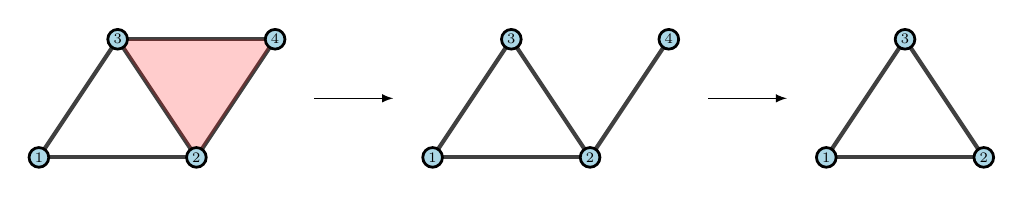
\begin{tikzpicture}
      \fill[opacity = 0.2, red] (2, 0) -- (1, 1.5) -- ( 3, 1.5) -- cycle; 
      \Vertex[x=0, y=0, size=0.25, fontscale=0.75, label=1]{v1}
      \Vertex[x=2, y=0, size=0.25, fontscale=0.75,label=2]{v2}
      \Vertex[x=1, y=1.5, size=0.25,fontscale=0.75, label=3]{v3}
      \Vertex[x=3, y=1.5, size=0.25,fontscale=0.75, label=4]{v4}
      \Edge(v1)(v2)
      \Edge(v1)(v3)
      \Edge(v2)(v3)
      \Edge(v2)(v4)
      \Edge(v3)(v4)

      \draw[-latex] ( 3.5, 0.75) -- (4.5, 0.75) ;

      \Vertex[x=5, y=0, size=0.25, fontscale=0.75, label=1]{v1}
      \Vertex[x=7, y=0, size=0.25, fontscale=0.75,label=2]{v2}
      \Vertex[x=6, y=1.5, size=0.25,fontscale=0.75, label=3]{v3}
      \Vertex[x=8, y=1.5, size=0.25,fontscale=0.75, label=4]{v4}
      \Edge(v1)(v2)
      \Edge(v1)(v3)
      \Edge(v2)(v3)
      \Edge(v2)(v4)

      \draw[-latex] ( 8.5, 0.75) -- (9.5, 0.75) ;

      \Vertex[x=10, y=0, size=0.25, fontscale=0.75, label=1]{v1}
      \Vertex[x=12, y=0, size=0.25, fontscale=0.75,label=2]{v2}
      \Vertex[x=11, y=1.5, size=0.25,fontscale=0.75, label=3]{v3}
      \Edge(v1)(v2)
      \Edge(v1)(v3)
      \Edge(v2)(v3)

\end{tikzpicture}
            \caption{Example of weakly collapsible but not collapsible simplicial complex \label{fig:weak_example}}
      \end{figure}
\end{example}

\begin{theorem}\label{thm:poly}
      Weak collapsibility of \( 2\)-skeleton \( \mc K \) is polynomially solvable.
\end{theorem}
\begin{proof}
      The \emph{greedy algorithm} for the collapsing sequence intuitively operates as follows: at each iteration perform any of possible collapses; in the absence of free edges, the complex should be considered not collapsible, \Cref{algo:greedy}. Clearly, such an algorithm runs polynomially with respect to the number of simplexes in \(\mc K\).
      % TODO:

      The failure of the greedy algorithm indicates the existence of a weakly collapsible complex \( \mc K \) such that the greedy algorithm gets stuck at a \( 2 \)-Core, which is avoidable for another possible order of collapses. Among all the counter exemplary complexes, let \( \mc K \) be a minimal one with respect to the number of triangles \( m_2 \). Then there exist a free edge \( \sigma \in \V 1 \) such that \( \mc K \backslash \{ \sigma \} \) is \emph{collapsible} and another \( \sigma' \in \V 2 \) such that \( \mc K \backslash \{ \sigma' \} \) is \emph{not collapsible}.

      Note that if \( \mc K \) is minimal then for any pair of free edges \( \sigma_1 \) and \( \sigma_2 \) belong to the same triangle: \( \tau(\sigma_1) = \tau(\sigma_2) \). Indeed, for any \( \tau(\sigma_1) \ne \tau(\sigma_2) \),  \( \mc K \backslash \{ \sigma_1, \sigma_2 \} = \mc K \backslash \{ \sigma_2, \sigma_1 \} \). Let \( \tau(\sigma_1) \ne \tau(\sigma_2) \) for at least one pair of \( \sigma_1 \) and \( \sigma_2 \); in our assumption, either both \( \mc K \backslash \{ \sigma_1 \} \) and \( \mc K \backslash \{ \sigma_2 \} \), only \( \mc K \backslash \{ \sigma_1 \}  \) or none are collapsible. In the former case either \( \mc K \backslash \{ \sigma_1 \} \) or \( \mc K \backslash \{ \sigma_2 \} \) is a smaller example of the complex satisfying the assumption, hence, violating the minimality. If only \( \mc K \backslash \{ \sigma_1 \} \) is collapsible, then \( \mc K \backslash \{ \sigma_2, \sigma_1 \}  \) is not collapsible; hence, \( \mc K \backslash \{ \sigma_1, \sigma_2 \} \) is not collapsible, so \( \mc K \backslash \{ \sigma_1 \} \) is a smaller example of a complex satisfying the assumption. Finally, if both \( \mc K \backslash \{ \sigma_1 \} \) and \( \mc K \backslash \{ \sigma_2 \} \) are collapsible, then for  known \( \sigma' \) such that \( \mc K \backslash \{ \sigma' \} \) is not collapsible, \( \tau(\sigma') \ne \tau(\sigma_1)\) or \( \tau(\sigma') \ne \tau(\sigma_2) \), which revisits the previous point.

      As a result, for \( \sigma \) ( \( \mc K \backslash \{ \sigma \} \) is collapsible) and for \( \sigma' \) ( \( \mc K \backslash \{ \sigma' \} \) is not collapsible ) it holds that \( \tau (\sigma) = \tau (\sigma') \Rightarrow  \sigma \cap \sigma' = \{ v \}  \), so after collapses \( \mc K  \{ \sigma \} \) and \( \mc K \backslash \{ \sigma' \} \) we arrive at two identical simplicial complexes modulo the hanging vertex irrelevant for the weak collapsibility. A simplicial complex can not be simultaneously collapsible and not collapsible, so the question of weak collapsibility can always be resolved by the greedy algorithm which has polynomial complexity.
\end{proof}

\begin{comment}
\blav
\begin{remark}
      The proof above is reminiscent of the one for polynomiality of \(d\)-collapsibility, \( d = 1\) or \( d = 2\), \cite{tancer2008dcollapse}, but bares significant differences: firstly, \( 2 \)-collapsibility allows collapses at \(\sigma: \; \dim \sigma \le 1\); secondly, in the scope of \cite{tancer2008dcollapse}, \( \tau(\sigma) = \sigma \) is allowed which affects (complicates) the proof.
\end{remark}
\elav


\begin{remark}
      If \( \mc K \) is weakly collapsible, then the number of triangles can not be higher than the number of edges, \( m_2 \le m_1 \), hence \( \mc K \) is \emph{necessarily sparse} and does not breach the gap up to \( m_2 = \mc O\left( m_1 \ln \left( 4 m_1 \right) \right) \).
\end{remark}
\end{comment}

\subsection{Computational cost of the greedy algorithm}

Let \( \mc K \) be a \(2\)-skeleton; let \( \Delta_\sigma \) be a set of triangles of \( \mc K \) containing the edge \( \sigma \), \( \Delta_\sigma = \{ t \mid  t \in \V 2  \text{ and } \sigma \in t \} \). Then the edge \( \sigma \) is free iff \( | \Delta_\sigma | = 1 \) and \( F = \{ \sigma \mid | \Delta_e | = 1  \} \) is a set of all free edges. Note that \( | \Delta_e | \le m_0 -2 = \mc O ( m_0  ) \).

\begin{algorithm}[h]
      \caption{ \texttt{GREEDY\_COLLAPSE}(\(\mc K\)):  greedy algorithm for the weak collapsibility
      \label{algo:greedy}}
      \begin{algorithmic}[1]
            \Require initial set of free edges \( F \), adjacency sets \(  \{ \Delta_{ \sigma_i } \}_{i=1}^{ m_1 } \)
             \State \( \Sigma = [ \; ] , \; \ds T = [ \; ] \) \Comment{ initialize the collapsing sequence}
             \While{ \( F \ne \vn \) \textbf{ and } \( \V 2 \ne \vn \) }
                  \State \( \sigma \gets \texttt{pop}( F ) \), \( \; \tau \gets \tau(\sigma)  \) \Comment{ pick a free edge \( \sigma \) }
                  \State \( \mc K \gets \mc K \backslash \{ \sigma \} \), \( \; \Sigma \gets [ \, \Sigma \;\; \sigma \, ] , \; \ds T \gets [ \ds T \; \tau ] \) \Comment{ \small \( \tau \) is a triangle being collapsed; \( \tau = [ \sigma, \sigma_1, \sigma_2 ] \) }
                  \State \( \Delta_{\sigma_1} \gets \Delta_{\sigma_1} \backslash \tau  \), \( \; \Delta_{\sigma_2} \gets \Delta_{\sigma_2} \backslash \tau  \) \Comment{ remove \( \tau \) from adjacency lists }
                  \State \( F \gets F \cup \{ \sigma_i \, |  \, i = 1, 2 \text{ and } | \Delta_{\sigma_i} | = 1 \}  \) \Comment{ update \( F \) if any of \( \sigma_1 \) or \( \sigma_2 \) has become free }
                  %\State \( \mc K \gets \mc K  \backslash \{ \sigma \} \) \Comment{ perform a collapse  }
             \EndWhile
             \State \Return \( \mc K, \, \Sigma, \, \ds T \)
      \end{algorithmic}
\end{algorithm}

The complexity of \Cref{algo:greedy} rests upon the precomputed \( \sigma \mapsto \Delta_\sigma \) structure that de-facto coincides with the boundary operator \( B_2 \) (assuming \( B_2 \) is stored as a sparse matrix, the adjacency structure describes its non-zero entries). Similarly, the initial \( F \) set can be computed alongside the construction of \( B_2 \) matrix. Another concession is needed for the complexity of the removal of elements from \( \Delta_{\sigma_i} \) and \( F \), which may vary from \( \mc O (1) \) on average up to guaranteed \( \log ( | \Delta_{\sigma_i} | ) \). As a result, given a pre-existing \( B_2 \) operator, \Cref{algo:greedy} runs linearly, \( \mc O ( m_1  )\), or almost linearly depending on the realisation, \( \mc O ( m_1 \log m_1 )\).


\todo{ Picture }


\section{ HeCS preconditioning }

\subsection{ Cholesky decomposition for weakly collapsible subcomplex }

\subsection{ Problem: precondition by subcomplex }


\subsection{ Optimal weights for subsampling }


\subsection{ Theorem on conditionality of a subcomplex }


\subsection{ The notion of the heavy collapsible subcomplex }


\subsection{ Algorithm and complexity }









\section{Benchmarking: triangulation}

\subsection{ Timings of algorithm and preconditioned application }

\subsection{ Conditionality and iterations }


\subsection{ Compare with shifted ichol }











%----------------------------------------------------------------------------------------
%	THESIS CONTENT - APPENDICES
%----------------------------------------------------------------------------------------

\addtocontents{toc}{\vspace{2em}} % Add a gap in the Contents, for aesthetics
%
\appendix % Cue to tell LaTeX that the following 'chapters' are Appendices

%% Include the appendices of the thesis as separate files from the Appendices folder
%% Uncomment the lines as you write the Appendices

%%----------------------------------------------------------------------------------------
%	Appendix A
%----------------------------------------------------------------------------------------
\chapter{Appendix Title Here}\label{app:appendixA}

\todo{Write your Appendix content here, if needed.}
%\input{./Appendices/AppendixB}
%\input{./Appendices/AppendixC}

%\addtocontents{toc}{\vspace{2em}} % Add a gap in the Contents, for aesthetics
%
%\backmatter

\clearpage

%----------------------------------------------------------------------------------------
%	BIBLIOGRAPHY
%----------------------------------------------------------------------------------------

\nocite{*}

\label{Bibliography}

\lhead{\emph{Bibliography}} % Change the page header to say "Bibliography"

\bibliographystyle{unsrtnat} % Use the "unsrtnat" BibTeX style for formatting the Bibliography

\bibliography{notes} % The references (bibliography) information are stored in the file named "Bibliography.bib"

\end{document}